\chapter{Learning with Perfect Bags: Addressing Hidden Stratification with Zero Labelled Data}\label{ch:paper3}
%%%%%%%%% ICML 2021 EXAMPLE LATEX SUBMISSION FILE %%%%%%%%%%%%%%%%%

%\documentclass{article}

%% Optional math commands from https://github.com/goodfeli/dlbook_notation.
%%%%%% NEW MATH DEFINITIONS %%%%%

\usepackage{amsmath,amsfonts,bm}

% Mark sections of captions for referring to divisions of figures
\newcommand{\figleft}{{\em (Left)}}
\newcommand{\figcenter}{{\em (Center)}}
\newcommand{\figright}{{\em (Right)}}
\newcommand{\figtop}{{\em (Top)}}
\newcommand{\figbottom}{{\em (Bottom)}}
\newcommand{\captiona}{{\em (a)}}
\newcommand{\captionb}{{\em (b)}}
\newcommand{\captionc}{{\em (c)}}
\newcommand{\captiond}{{\em (d)}}

% Highlight a newly defined term
\newcommand{\newterm}[1]{{\bf #1}}


% Figure reference, lower-case.
\def\figref#1{figure~\ref{#1}}
% Figure reference, capital. For start of sentence
\def\Figref#1{Figure~\ref{#1}}
\def\twofigref#1#2{figures \ref{#1} and \ref{#2}}
\def\quadfigref#1#2#3#4{figures \ref{#1}, \ref{#2}, \ref{#3} and \ref{#4}}
% Section reference, lower-case.
\def\secref#1{section~\ref{#1}}
% Section reference, capital.
\def\Secref#1{Section~\ref{#1}}
% Reference to two sections.
\def\twosecrefs#1#2{sections \ref{#1} and \ref{#2}}
% Reference to three sections.
\def\secrefs#1#2#3{sections \ref{#1}, \ref{#2} and \ref{#3}}
% Appendix reference, lower-case.
\def\appref#1{appendix~\ref{#1}}
% Appendix reference, capital.
\def\Appref#1{Appendix~\ref{#1}}
% Reference to an equation, lower-case.
\def\eqref#1{equation~\ref{#1}}
% Reference to an equation, upper case
\def\Eqref#1{Equation~\ref{#1}}
% A raw reference to an equation---avoid using if possible
\def\plaineqref#1{\ref{#1}}
% Reference to a chapter, lower-case.
\def\chapref#1{chapter~\ref{#1}}
% Reference to a Chapter, upper case.
\def\Chapref#1{Chapter~\ref{#1}}
\def\twochaprefs#1#2{chapters \ref{#1} and \ref{#2}}
% Reference to a range of chapters
\def\rangechapref#1#2{chapters \ref{#1}--\ref{#2}}
% Reference to a range of chapters, upper case
\def\Rangechapref#1#2{Chapters \ref{#1}--\ref{#2}}
% Reference to an algorithm, lower-case.
\def\algref#1{algorithm~\ref{#1}}
% Reference to an algorithm, upper case.
\def\Algref#1{Algorithm~\ref{#1}}
\def\twoalgref#1#2{algorithms \ref{#1} and \ref{#2}}
\def\Twoalgref#1#2{Algorithms \ref{#1} and \ref{#2}}
% Reference to a part, lower case
\def\partref#1{part~\ref{#1}}
% Reference to a part, upper case
\def\Partref#1{Part~\ref{#1}}
\def\twopartref#1#2{parts \ref{#1} and \ref{#2}}

\def\ceil#1{\lceil #1 \rceil}
\def\floor#1{\lfloor #1 \rfloor}
\def\1{\bm{1}}
\newcommand{\train}{\mathcal{D}}
\newcommand{\valid}{\mathcal{D_{\mathrm{valid}}}}
\newcommand{\test}{\mathcal{D_{\mathrm{test}}}}

\def\eps{{\epsilon}}


% Random variables
\def\reta{{\textnormal{$\eta$}}}
\def\ra{{\textnormal{a}}}
\def\rb{{\textnormal{b}}}
\def\rc{{\textnormal{c}}}
\def\rd{{\textnormal{d}}}
\def\re{{\textnormal{e}}}
\def\rf{{\textnormal{f}}}
\def\rg{{\textnormal{g}}}
\def\rh{{\textnormal{h}}}
\def\ri{{\textnormal{i}}}
\def\rj{{\textnormal{j}}}
\def\rk{{\textnormal{k}}}
\def\rl{{\textnormal{l}}}
% rm is already a command, just don't name any random variables m
\def\rn{{\textnormal{n}}}
\def\ro{{\textnormal{o}}}
\def\rp{{\textnormal{p}}}
\def\rq{{\textnormal{q}}}
\def\rr{{\textnormal{r}}}
\def\rs{{\textnormal{s}}}
\def\rt{{\textnormal{t}}}
\def\ru{{\textnormal{u}}}
\def\rv{{\textnormal{v}}}
\def\rw{{\textnormal{w}}}
\def\rx{{\textnormal{x}}}
\def\ry{{\textnormal{y}}}
\def\rz{{\textnormal{z}}}

% Random vectors
\def\rvepsilon{{\mathbf{\epsilon}}}
\def\rvtheta{{\mathbf{\theta}}}
\def\rva{{\mathbf{a}}}
\def\rvb{{\mathbf{b}}}
\def\rvc{{\mathbf{c}}}
\def\rvd{{\mathbf{d}}}
\def\rve{{\mathbf{e}}}
\def\rvf{{\mathbf{f}}}
\def\rvg{{\mathbf{g}}}
\def\rvh{{\mathbf{h}}}
\def\rvu{{\mathbf{i}}}
\def\rvj{{\mathbf{j}}}
\def\rvk{{\mathbf{k}}}
\def\rvl{{\mathbf{l}}}
\def\rvm{{\mathbf{m}}}
\def\rvn{{\mathbf{n}}}
\def\rvo{{\mathbf{o}}}
\def\rvp{{\mathbf{p}}}
\def\rvq{{\mathbf{q}}}
\def\rvr{{\mathbf{r}}}
\def\rvs{{\mathbf{s}}}
\def\rvt{{\mathbf{t}}}
\def\rvu{{\mathbf{u}}}
\def\rvv{{\mathbf{v}}}
\def\rvw{{\mathbf{w}}}
\def\rvx{{\mathbf{x}}}
\def\rvy{{\mathbf{y}}}
\def\rvz{{\mathbf{z}}}

% Elements of random vectors
\def\erva{{\textnormal{a}}}
\def\ervb{{\textnormal{b}}}
\def\ervc{{\textnormal{c}}}
\def\ervd{{\textnormal{d}}}
\def\erve{{\textnormal{e}}}
\def\ervf{{\textnormal{f}}}
\def\ervg{{\textnormal{g}}}
\def\ervh{{\textnormal{h}}}
\def\ervi{{\textnormal{i}}}
\def\ervj{{\textnormal{j}}}
\def\ervk{{\textnormal{k}}}
\def\ervl{{\textnormal{l}}}
\def\ervm{{\textnormal{m}}}
\def\ervn{{\textnormal{n}}}
\def\ervo{{\textnormal{o}}}
\def\ervp{{\textnormal{p}}}
\def\ervq{{\textnormal{q}}}
\def\ervr{{\textnormal{r}}}
\def\ervs{{\textnormal{s}}}
\def\ervt{{\textnormal{t}}}
\def\ervu{{\textnormal{u}}}
\def\ervv{{\textnormal{v}}}
\def\ervw{{\textnormal{w}}}
\def\ervx{{\textnormal{x}}}
\def\ervy{{\textnormal{y}}}
\def\ervz{{\textnormal{z}}}

% Random matrices
\def\rmA{{\mathbf{A}}}
\def\rmB{{\mathbf{B}}}
\def\rmC{{\mathbf{C}}}
\def\rmD{{\mathbf{D}}}
\def\rmE{{\mathbf{E}}}
\def\rmF{{\mathbf{F}}}
\def\rmG{{\mathbf{G}}}
\def\rmH{{\mathbf{H}}}
\def\rmI{{\mathbf{I}}}
\def\rmJ{{\mathbf{J}}}
\def\rmK{{\mathbf{K}}}
\def\rmL{{\mathbf{L}}}
\def\rmM{{\mathbf{M}}}
\def\rmN{{\mathbf{N}}}
\def\rmO{{\mathbf{O}}}
\def\rmP{{\mathbf{P}}}
\def\rmQ{{\mathbf{Q}}}
\def\rmR{{\mathbf{R}}}
\def\rmS{{\mathbf{S}}}
\def\rmT{{\mathbf{T}}}
\def\rmU{{\mathbf{U}}}
\def\rmV{{\mathbf{V}}}
\def\rmW{{\mathbf{W}}}
\def\rmX{{\mathbf{X}}}
\def\rmY{{\mathbf{Y}}}
\def\rmZ{{\mathbf{Z}}}

% Elements of random matrices
\def\ermA{{\textnormal{A}}}
\def\ermB{{\textnormal{B}}}
\def\ermC{{\textnormal{C}}}
\def\ermD{{\textnormal{D}}}
\def\ermE{{\textnormal{E}}}
\def\ermF{{\textnormal{F}}}
\def\ermG{{\textnormal{G}}}
\def\ermH{{\textnormal{H}}}
\def\ermI{{\textnormal{I}}}
\def\ermJ{{\textnormal{J}}}
\def\ermK{{\textnormal{K}}}
\def\ermL{{\textnormal{L}}}
\def\ermM{{\textnormal{M}}}
\def\ermN{{\textnormal{N}}}
\def\ermO{{\textnormal{O}}}
\def\ermP{{\textnormal{P}}}
\def\ermQ{{\textnormal{Q}}}
\def\ermR{{\textnormal{R}}}
\def\ermS{{\textnormal{S}}}
\def\ermT{{\textnormal{T}}}
\def\ermU{{\textnormal{U}}}
\def\ermV{{\textnormal{V}}}
\def\ermW{{\textnormal{W}}}
\def\ermX{{\textnormal{X}}}
\def\ermY{{\textnormal{Y}}}
\def\ermZ{{\textnormal{Z}}}

% Vectors
\def\vzero{{\bm{0}}}
\def\vone{{\bm{1}}}
\def\vmu{{\bm{\mu}}}
\def\vtheta{{\bm{\theta}}}
\def\va{{\bm{a}}}
\def\vb{{\bm{b}}}
\def\vc{{\bm{c}}}
\def\vd{{\bm{d}}}
\def\ve{{\bm{e}}}
\def\vf{{\bm{f}}}
\def\vg{{\bm{g}}}
\def\vh{{\bm{h}}}
\def\vi{{\bm{i}}}
\def\vj{{\bm{j}}}
\def\vk{{\bm{k}}}
\def\vl{{\bm{l}}}
\def\vm{{\bm{m}}}
\def\vn{{\bm{n}}}
\def\vo{{\bm{o}}}
\def\vp{{\bm{p}}}
\def\vq{{\bm{q}}}
\def\vr{{\bm{r}}}
\def\vs{{\bm{s}}}
\def\vt{{\bm{t}}}
\def\vu{{\bm{u}}}
\def\vv{{\bm{v}}}
\def\vw{{\bm{w}}}
\def\vx{{\bm{x}}}
\def\vy{{\bm{y}}}
\def\vz{{\bm{z}}}

% Elements of vectors
\def\evalpha{{\alpha}}
\def\evbeta{{\beta}}
\def\evepsilon{{\epsilon}}
\def\evlambda{{\lambda}}
\def\evomega{{\omega}}
\def\evmu{{\mu}}
\def\evpsi{{\psi}}
\def\evsigma{{\sigma}}
\def\evtheta{{\theta}}
\def\eva{{a}}
\def\evb{{b}}
\def\evc{{c}}
\def\evd{{d}}
\def\eve{{e}}
\def\evf{{f}}
\def\evg{{g}}
\def\evh{{h}}
\def\evi{{i}}
\def\evj{{j}}
\def\evk{{k}}
\def\evl{{l}}
\def\evm{{m}}
\def\evn{{n}}
\def\evo{{o}}
\def\evp{{p}}
\def\evq{{q}}
\def\evr{{r}}
\def\evs{{s}}
\def\evt{{t}}
\def\evu{{u}}
\def\evv{{v}}
\def\evw{{w}}
\def\evx{{x}}
\def\evy{{y}}
\def\evz{{z}}

% Matrix
\def\mA{{\bm{A}}}
\def\mB{{\bm{B}}}
\def\mC{{\bm{C}}}
\def\mD{{\bm{D}}}
\def\mE{{\bm{E}}}
\def\mF{{\bm{F}}}
\def\mG{{\bm{G}}}
\def\mH{{\bm{H}}}
\def\mI{{\bm{I}}}
\def\mJ{{\bm{J}}}
\def\mK{{\bm{K}}}
\def\mL{{\bm{L}}}
\def\mM{{\bm{M}}}
\def\mN{{\bm{N}}}
\def\mO{{\bm{O}}}
\def\mP{{\bm{P}}}
\def\mQ{{\bm{Q}}}
\def\mR{{\bm{R}}}
\def\mS{{\bm{S}}}
\def\mT{{\bm{T}}}
\def\mU{{\bm{U}}}
\def\mV{{\bm{V}}}
\def\mW{{\bm{W}}}
\def\mX{{\bm{X}}}
\def\mY{{\bm{Y}}}
\def\mZ{{\bm{Z}}}
\def\mBeta{{\bm{\beta}}}
\def\mPhi{{\bm{\Phi}}}
\def\mLambda{{\bm{\Lambda}}}
\def\mSigma{{\bm{\Sigma}}}

% % Tensor
% \DeclareMathAlphabet{\mathsfit}{\encodingdefault}{\sfdefault}{m}{sl}
% \SetMathAlphabet{\mathsfit}{bold}{\encodingdefault}{\sfdefault}{bx}{n}
% \newcommand{\tens}[1]{\bm{\mathsfit{#1}}}
% \def\tA{{\tens{A}}}
% \def\tB{{\tens{B}}}
% \def\tC{{\tens{C}}}
% \def\tD{{\tens{D}}}
% \def\tE{{\tens{E}}}
% \def\tF{{\tens{F}}}
% \def\tG{{\tens{G}}}
% \def\tH{{\tens{H}}}
% \def\tI{{\tens{I}}}
% \def\tJ{{\tens{J}}}
% \def\tK{{\tens{K}}}
% \def\tL{{\tens{L}}}
% \def\tM{{\tens{M}}}
% \def\tN{{\tens{N}}}
% \def\tO{{\tens{O}}}
% \def\tP{{\tens{P}}}
% \def\tQ{{\tens{Q}}}
% \def\tR{{\tens{R}}}
% \def\tS{{\tens{S}}}
% \def\tT{{\tens{T}}}
% \def\tU{{\tens{U}}}
% \def\tV{{\tens{V}}}
% \def\tW{{\tens{W}}}
% \def\tX{{\tens{X}}}
% \def\tY{{\tens{Y}}}
% \def\tZ{{\tens{Z}}}


% Graph
\def\gA{{\mathcal{A}}}
\def\gB{{\mathcal{B}}}
\def\gC{{\mathcal{C}}}
\def\gD{{\mathcal{D}}}
\def\gE{{\mathcal{E}}}
\def\gF{{\mathcal{F}}}
\def\gG{{\mathcal{G}}}
\def\gH{{\mathcal{H}}}
\def\gI{{\mathcal{I}}}
\def\gJ{{\mathcal{J}}}
\def\gK{{\mathcal{K}}}
\def\gL{{\mathcal{L}}}
\def\gM{{\mathcal{M}}}
\def\gN{{\mathcal{N}}}
\def\gO{{\mathcal{O}}}
\def\gP{{\mathcal{P}}}
\def\gQ{{\mathcal{Q}}}
\def\gR{{\mathcal{R}}}
\def\gS{{\mathcal{S}}}
\def\gT{{\mathcal{T}}}
\def\gU{{\mathcal{U}}}
\def\gV{{\mathcal{V}}}
\def\gW{{\mathcal{W}}}
\def\gX{{\mathcal{X}}}
\def\gY{{\mathcal{Y}}}
\def\gZ{{\mathcal{Z}}}

% Sets
\def\sA{{\mathbb{A}}}
\def\sB{{\mathbb{B}}}
\def\sC{{\mathbb{C}}}
\def\sD{{\mathbb{D}}}
% Don't use a set called E, because this would be the same as our symbol
% for expectation.
\def\sF{{\mathbb{F}}}
\def\sG{{\mathbb{G}}}
\def\sH{{\mathbb{H}}}
\def\sI{{\mathbb{I}}}
\def\sJ{{\mathbb{J}}}
\def\sK{{\mathbb{K}}}
\def\sL{{\mathbb{L}}}
\def\sM{{\mathbb{M}}}
\def\sN{{\mathbb{N}}}
\def\sO{{\mathbb{O}}}
\def\sP{{\mathbb{P}}}
\def\sQ{{\mathbb{Q}}}
\def\sR{{\mathbb{R}}}
\def\sS{{\mathbb{S}}}
\def\sT{{\mathbb{T}}}
\def\sU{{\mathbb{U}}}
\def\sV{{\mathbb{V}}}
\def\sW{{\mathbb{W}}}
\def\sX{{\mathbb{X}}}
\def\sY{{\mathbb{Y}}}
\def\sZ{{\mathbb{Z}}}

% Entries of a matrix
\def\emLambda{{\Lambda}}
\def\emA{{A}}
\def\emB{{B}}
\def\emC{{C}}
\def\emD{{D}}
\def\emE{{E}}
\def\emF{{F}}
\def\emG{{G}}
\def\emH{{H}}
\def\emI{{I}}
\def\emJ{{J}}
\def\emK{{K}}
\def\emL{{L}}
\def\emM{{M}}
\def\emN{{N}}
\def\emO{{O}}
\def\emP{{P}}
\def\emQ{{Q}}
\def\emR{{R}}
\def\emS{{S}}
\def\emT{{T}}
\def\emU{{U}}
\def\emV{{V}}
\def\emW{{W}}
\def\emX{{X}}
\def\emY{{Y}}
\def\emZ{{Z}}
\def\emSigma{{\Sigma}}

% entries of a tensor
% Same font as tensor, without \bm wrapper
% \newcommand{\etens}[1]{\mathsfit{#1}}
% \def\etLambda{{\etens{\Lambda}}}
% \def\etA{{\etens{A}}}
% \def\etB{{\etens{B}}}
% \def\etC{{\etens{C}}}
% \def\etD{{\etens{D}}}
% \def\etE{{\etens{E}}}
% \def\etF{{\etens{F}}}
% \def\etG{{\etens{G}}}
% \def\etH{{\etens{H}}}
% \def\etI{{\etens{I}}}
% \def\etJ{{\etens{J}}}
% \def\etK{{\etens{K}}}
% \def\etL{{\etens{L}}}
% \def\etM{{\etens{M}}}
% \def\etN{{\etens{N}}}
% \def\etO{{\etens{O}}}
% \def\etP{{\etens{P}}}
% \def\etQ{{\etens{Q}}}
% \def\etR{{\etens{R}}}
% \def\etS{{\etens{S}}}
% \def\etT{{\etens{T}}}
% \def\etU{{\etens{U}}}
% \def\etV{{\etens{V}}}
% \def\etW{{\etens{W}}}
% \def\etX{{\etens{X}}}
% \def\etY{{\etens{Y}}}
% \def\etZ{{\etens{Z}}}

% The true underlying data generating distribution
\newcommand{\pdata}{p_{\rm{data}}}
% The empirical distribution defined by the training set
\newcommand{\ptrain}{\hat{p}_{\rm{data}}}
\newcommand{\Ptrain}{\hat{P}_{\rm{data}}}
% The model distribution
\newcommand{\pmodel}{p_{\rm{model}}}
\newcommand{\Pmodel}{P_{\rm{model}}}
\newcommand{\ptildemodel}{\tilde{p}_{\rm{model}}}
% Stochastic autoencoder distributions
\newcommand{\pencode}{p_{\rm{encoder}}}
\newcommand{\pdecode}{p_{\rm{decoder}}}
\newcommand{\precons}{p_{\rm{reconstruct}}}

\newcommand{\laplace}{\mathrm{Laplace}} % Laplace distribution

\newcommand{\E}{\mathbb{E}}
\newcommand{\Ls}{\mathcal{L}}
\newcommand{\R}{\mathbb{R}}
\newcommand{\emp}{\tilde{p}}
\newcommand{\lr}{\alpha}
\newcommand{\reg}{\lambda}
\newcommand{\rect}{\mathrm{rectifier}}
\newcommand{\softmax}{\mathrm{softmax}}
\newcommand{\sigmoid}{\sigma}
\newcommand{\softplus}{\zeta}
\newcommand{\KL}{D_{\mathrm{KL}}}
\newcommand{\Var}{\mathrm{Var}}
\newcommand{\standarderror}{\mathrm{SE}}
\newcommand{\Cov}{\mathrm{Cov}}
% Wolfram Mathworld says $L^2$ is for function spaces and $\ell^2$ is for vectors
% But then they seem to use $L^2$ for vectors throughout the site, and so does
% wikipedia.
\newcommand{\normlzero}{L^0}
\newcommand{\normlone}{L^1}
\newcommand{\normltwo}{L^2}
\newcommand{\normlp}{L^p}
\newcommand{\normmax}{L^\infty}

\newcommand{\parents}{Pa} % See usage in notation.tex. Chosen to match Daphne's book.

\DeclareMathOperator*{\argmax}{arg\,max}
\DeclareMathOperator*{\argmin}{arg\,min}

\DeclareMathOperator{\sign}{sign}
\DeclareMathOperator{\Tr}{Tr}
\let\ab\allowbreak


%% Recommended, but optional, packages for figures and better typesetting:
%\usepackage{microtype}
%\usepackage{graphicx}
%\usepackage{wrapfig}
%\usepackage{caption}
%\usepackage{subcaption}
%\usepackage{booktabs} % for professional tables
%\usepackage{amsfonts}       % blackboard math symbols
%\usepackage{amsmath}
%\usepackage{amssymb}
%\usepackage{amsthm}
%\usepackage{nicefrac}       % compact symbols for 1/2, etc.
%\usepackage{xcolor}         %for colouring the text on colourMNIST
%\usepackage{comment}
%\usepackage{enumitem}
%\newtheorem{prop}{Proposition}
%\newcommand{\Xcal}{\mathcal{X}}
%\newcommand{\Bcal}{\mathcal{B}}
%\newcommand{\Ycal}{\mathcal{Y}}
%\newcommand{\Scal}{\mathcal{S}}
%\newcommand{\Lcal}{\mathcal{L}}
%\newcommand{\Dcal}{\mathcal{D}}
%\newcommand{\ie}{i.\,e.}
%\newcommand{\Ie}{I.\,e.}
%\newcommand{\eg}{e.\,g.}
%\newcommand{\Eg}{E.\,g.}

%% hyperref makes hyperlinks in the resulting PDF.
%% If your build breaks (sometimes temporarily if a hyperlink spans a page)
%% please comment out the following usepackage line and replace
%% \usepackage{icml2021} with \usepackage[nohyperref]{icml2021} above.
%\usepackage{hyperref}

%% Attempt to make hyperref and algorithmic work together better:
%\newcommand{\theHalgorithm}{\arabic{algorithm}}

%% Use the following line for the initial blind version submitted for review:
%\usepackage{icml2021}

%% If accepted, instead use the following line for the camera-ready submission:
%%\usepackage[accepted]{icml2021}

%% The \icmltitle you define below is probably too long as a header.
%% Therefore, a short form for the running title is supplied here:
%\icmltitlerunning{Learning with Perfect Bags}

%\begin{document}

%\twocolumn[
%\icmltitle{Learning with Perfect Bags:\\
%Addressing Hidden Stratification with Zero Labelled Data}

%% It is OKAY to include author information, even for blind
%% submissions: the style file will automatically remove it for you
%% unless you've provided the [accepted] option to the icml2021
%% package.

%% List of affiliations: The first argument should be a (short)
%% identifier you will use later to specify author affiliations
%% Academic affiliations should list Department, University, City, Region, Country
%% Industry affiliations should list Company, City, Region, Country

%% You can specify symbols, otherwise they are numbered in order.
%% Ideally, you should not use this facility. Affiliations will be numbered
%% in order of appearance and this is the preferred way.
%\icmlsetsymbol{equal}{*}

%\begin{icmlauthorlist}
%\icmlauthor{Aeiau Zzzz}{equal,to}
%\icmlauthor{Bauiu C.~Yyyy}{equal,to,goo}
%\icmlauthor{Cieua Vvvvv}{goo}
%\icmlauthor{Iaesut Saoeu}{ed}
%\icmlauthor{Fiuea Rrrr}{to}
%\icmlauthor{Tateu H.~Yasehe}{ed,to,goo}
%\icmlauthor{Aaoeu Iasoh}{goo}
%\icmlauthor{Buiui Eueu}{ed}
%\icmlauthor{Aeuia Zzzz}{ed}
%\icmlauthor{Bieea C.~Yyyy}{to,goo}
%\icmlauthor{Teoau Xxxx}{ed}
%\icmlauthor{Eee Pppp}{ed}
%\end{icmlauthorlist}

%\icmlaffiliation{to}{Department of Computation, University of Torontoland, Torontoland, Canada}
%\icmlaffiliation{goo}{Googol ShallowMind, New London, Michigan, USA}
%\icmlaffiliation{ed}{School of Computation, University of Edenborrow, Edenborrow, United Kingdom}

%\icmlcorrespondingauthor{Cieua Vvvvv}{c.vvvvv@googol.com}
%\icmlcorrespondingauthor{Eee Pppp}{ep@eden.co.uk}

%% You may provide any keywords that you
%% find helpful for describing your paper; these are used to populate
%% the "keywords" metadata in the PDF but will not be shown in the document
%\icmlkeywords{semi-supervised learning, dataset bias}

%\vskip 0.3in
%]

%% this must go after the closing bracket ] following \twocolumn[ ...

%% This command actually creates the footnote in the first column
%% listing the affiliations and the copyright notice.
%% The command takes one argument, which is text to display at the start of the footnote.
%% The \icmlEqualContribution command is standard text for equal contribution.
%% Remove it (just {}) if you do not need this facility.

%%\printAffiliationsAndNotice{}  % leave blank if no need to mention equal contribution
%\printAffiliationsAndNotice{\icmlEqualContribution} % otherwise use the standard text.

%\icmltitle{Learning with Perfect Bags:\\
%Addressing Hidden Stratification with Zero Labelled Data}
\textsc{Authors}:
Thomas Kehrenberg$^1$, Myles Bartlett$^1$, Novi Quadrianto$^1$ and Vik\-to\-riia Shar\-man\-s\-ka$^1$ \\
\textsc{Affiliations}:\\
$^1$ Predictive Analytics Lab (PAL), University of Sussex, Brighton, UK\\
% \textsc{Conference}:\;\; Submitted to \textit{International Conference on Machine Learning} (ICML), 2021 \\
% \textsc{DOI}:\;\;10.3389/frai.2020.00033
\textsc{Note}:\;\; The appendix has been included as section~\ref{sec:zsf-appendix}.

\section{Abstract}
Machine learning models are typically trained to optimise global metrics such as average classification accuracy. 
%
Hidden stratification arises when the trained models have high average performance over classes but exhibit highly variable performance across different hidden subgroups.
%
In this paper, we consider the setting where the hidden stratification has zero class-labelled data for some subgroups. 
As an illustration, we have digit images labelled as ``two'' or ``four'', each class comprises ``green'' and ``purple'' subgroups.
%
Challengingly, in the training data, twos can be any colour, but all fours are green. 
%
Without additional knowledge, it is impossible to directly control the discrepancy of the classifier’s statistics for the hidden subgroups. 
%
We develop a disentanglement algorithm that decomposes a data representation into a component that captures the subgrouping factors and a component that is invariant to them based on unlabelled (deployment) data. 
%
We cluster the unlabelled data, and equalise the cluster sizes to form ``perfect bags'' with respect to class and subgroup information.
%
We cast the problem of disentangling as one of distribution matching and propose an adversarial learning approach.
%
%We introduce a new discriminator loss, inspired by set-classification, to distinguish a batch of perfect bags from non-perfect ones based on a learnable attention mechanism. 
%
Unlike sample-based models, we advance a discriminator to assign scores at the level of bags of samples, with a bag being deemed authentic if was drawn from the unbiased distribution. 
%a parametric approach based on adversarial learning. 
%We take inspiration from set-classification and equip the discriminator with a learnable attention mechanism to model interdependencies between samples in a bag.
%
We evaluate our approach on several classification benchmarks and show that it is indeed possible to account for zero-label hidden stratification.
% \end{abstract}

\section{Introduction}%
\label{sec:introduction}
Machine learning has been deployed in safety-critical applications such as medicine \citep[e.g.][]{DunYiLanReetal19}, and socially important contexts such as the allocation of healthcare, education, and credit \citep[e.g.][]{HurAde17,RagBarKleLev20}.
%
Efficiency can be improved, costs can be reduced, and personalisation of services and products can be greatly enhanced -- these are some of the drivers for the widespread development and deployment of machine learning algorithms. 
%

Algorithms such as classifiers, however, are trained from large amount of labelled data, and are typically trained to optimise \emph{global} metrics such as average classification accuracy.
%
% \begin{figure*}[t]
% \centering
% \includegraphics[width=0.6\textwidth,page=2]{paper3/figures/ideal.pdf}
% \caption{Overview of the zero-shot stratification problem. Training dataset (pairs of input data $x$ and class label $y$) will only contain data points that are labelled ``yes'' by the decision policy. This systematic bias might result in a subgroup(s) to have zero labelled data (in the example above, ``married'' subgroup has zero labelled data). The subgrouping information $s$ is unavailable/unlabelled at deployment time, and is only partially labelled at train time.}
% \vspace{-0.5cm}
% \label{fig:censoring}
% \end{figure*}
In many real-world classification tasks, each labelled class consists of multiple semantically distinct subclasses, or subgroups.
For example, the ``dog'' class label can have finer-grained intra-class variations, such as ``dog indoor'' and ``dog outdoor''.
%
This finer-grained subgrouping information is typically unavailable/unlabelled \citep[e.g.][]{SohDunAngGuetal20,nam2020learning}.
%
The standard training process brings about two inter-connected challenges: a) classifiers often under-perform on important hidden subgroups (\emph{hidden stratification}) \citep{RayDunCarRe20,SohDunAngGuetal20};
and b) \emph{systematic bias}~\citep{kallus2018residual} affects whether or not entire collections of data points appear in the training dataset,
and can make the classifier unprepared for treating those subgroups in the eventual deployment setting
% and can hamper attempts to correct for bias in the eventual deployment data
(\emph{residual bias}). %\cite{kallus2018residual}.

We are interested in hidden stratification in which, for some of the subgroups, labelled training data is only available with a certain outcome, or labelled training samples are not available at all, due to systematic bias.
This can be seen as a strong sampling bias.
%
For instance, data on loan defaults can only be collected on those loan
applicants who were approved in the past \citep{kallus2018residual}.
%
Here a loan decision policy specifies whether an individual will be included in the training dataset.
%
Individuals can be thought of as belonging to a specific subgroup such as ``married'' or ``not married'' and systematic bias produced by a historical decision policy may result in the ``not married'' subgroup having poor, or altogether non-existent, representation.
%For instance, a medical imaging model trained to classify between ``benign'' and ``abnormal'' lesions may achieve high overall performance, yet consistently mislabel a rare but critical abnormal subgroup as ``benign'' \cite{DunYiLanReetal19}.
%
%Each class actually composes of ``no-patch'' and ``patch'' hidden subgroups, and the ``no-patch'' subgroup is further splitted into “histopathology” and “non-histopathology”.
%
%A past decision policy of \emph{not} requiring histopathology (biopsy \& pathologist referral) specifies whether an individual will be included in the training dataset.
%
%This systematic bias might lead to the no-patch subgroup to have thin or non-existent labelled data.
%
We formalise this stratification problem as a data setting where a decision policy can lead to one or more subgroups having no labelled data.

To address the problem of subgroup bias, this paper focuses on learning subgroup-invariant representations in the presence of zero-label stratification.
These representations can then be used to train a classifier that generalises to the deployment setting which does not exhibit the bias of the training set.
%
To learn the representation, a form of supervision is needed.
Our source of supervision is motivated by the observation that we want to deploy our classifier to the eventual real-world population.
%
A deployment set will contain data points from all subgroups.
%
We thus consider the setting where \emph{unlabelled} data is available for learning representations that disentangle the subgroup membership from the class membership. We note, however, that the test set could be used for this purpose in a transductive setting.

We aim to convert our unlabelled data into a collection of \emph{perfect bags} \citep{kleinberg2016inherent,chouldechova2017fair}, \ie\ sample sets in which the class label $y$ and subgroup label $s$ are independent (\ie\ $y\perp s$).
Making use of the terminology from \emph{multiple-instance learning}, our batches comprise a certain number of bags which are a collection of samples.
%
We will then use these perfect bags as the inductive bias for learning the disentangled representations. 
The disentangling procedure is thus in a sense \emph{supervised}.
%
How can we construct these perfect bags in the absence of any labelled data?
%
We assume that the number of subgroups is known \emph{a priori}\footnote{Relaxing this assumption represents a clear avenue for future work. We elaborate this in the limitation and intended use sec.~\ref{sec:limitations}.}. 
%We elaborate this further in our experiments and discussions sections.}.
%corresponding to the diverse demographic groups in the real-world population in which our machine learning system will be deployed. 
%
We then apply unsupervised k-means clustering, or a \emph{semi}-supervised clustering based on rank statistics; the latter allows incorporating annotations from the training data when forming the clusters.
%
Once the clusters have been found, we can sample from each cluster at an equal rate to form balanced (\ie\,\emph{perfect}) bags and use them as input for learning a disentangled representation. 
%
%See fig. \ref{fig:teaser} for an overview of our learning with invisible demographic framework.
We cast the problem of disentangling as one of distribution matching and propose an adversarial learning approach.
%a parametric approach based on adversarial learning. 
In the standard GAN setting, the discriminator assigns a score to each sample corresponding to the perceived probability that it was drawn from the true data distribution, and not the generator's.
In contrast, we train a discriminator to assign scores at the level of bags of samples, with a bag being deemed authentic if it was drawn from the originally unbiased distribution and not the de-biased one (with the de-biaser playing the role of the generator). To do so, we take inspiration from set-classification and multiple-instance learning and equip the discriminator with a learnable attention mechanism to model interdependencies between samples in a bag.

Specifically, our paper provides the following contributions:
\begin{enumerate}
    \item An example of systematic bias leading to one or more subgroups having \emph{zero labelled data}.
    \item Applying clustering methods to the task of transforming an \emph{unlabelled dataset} into perfect bags.
    \item Theoretical and experimental justification that the disentangling model with \emph{the perfect bag as an inductive bias} provides a well-disentangled representation, where one component captures the subgrouping factors and another component is invariant to them.
    \item A new parametric approach to disentangling that combines elements from adversarial learning and set-classification to guide an encoder network towards the goal of producing encodings invariant to the source distribution and thereby the subgroup factors in which source distributions differ.
\end{enumerate}

\section{Related work.}
We describe related work in two areas: zero-shot learning and semi-su\-per\-vi\-sed learning.
%and disentangled representation learning. 

\subsection{On zero-shot learning.}
The setting with incomplete training data, where we aim to account for seen and unseen outcomes is also known as \emph{generalised zero-shot learning}. 
Traditionally, zero-shot learning transfers knowledge from classes for which we have training data to classes for which we do not, via auxiliary knowledge, e.g. via prototype examples \citep{larochelle2008}, intermediate class description such as semantic attributes \citep{lampert2009, xian2018zero}, word2vec embeddings \citep{bucher2019}. 
Our method similarly uses a collection of perfect bags as a source of auxiliary knowledge but in contrast to generalised zero-shot learning, our perfect bag is an unlabelled pool of data, where class descriptions are unknown. 

\subsection{On semi-supervised learning.} 
\citet{wick2019unlocking} proposed a semi-supervised method that can successfully harness unlabelled data to correct for the selection bias and label bias in the training data.
%
The unlabelled data, despite not containing the class label $y$, \emph{is} labelled in terms of the subgroup label $s$. 
%
Our setting is significantly harder because there is no label information about $y$ and $s$ in the perfect bag.

\subsection{On disentangled representations learning.}%
\label{ssec:on-disentangled-representation-learning}
\citet{locatello2019fairness} suggested that disentanglement in representation learning may be a useful property to remove algorithmic bias when subgroup information is not observed.
%
In order for disentangled representations to reduce algorithmic bias without the knowledge of subgroup label $s$, they have to assume that the class label $y$ and the subgroup label $s$ are independent, i.e. $y\perp s$.
%
Though, in many real-world tasks, the variable $s$ is correlated with the variable $y$, and therefore unsupervised methods are not suitable  \citep{jaiswal2018unsupervised,JaiWuAbdNat19}. 
%
Indeed, experiments in \citet{locatello2019fairness} were wholly done with procedurally generated synthetic datasets involving 2D and 3D shapes. 
%
Without some supervision or inductive bias, disentangled representation methods would not solve the issue of algorithmic fairness with invisible demographics \citep{locatello2019challenging}. 
\citet{locatello2020weakly} suggest that that it is possible to learn disentangled representations
with contrasting pairs that share at least one of the underlying factors but differ in some.
Here, the difference between the pairs acts as the supervision signal.

%\begin{wrapfigure}{!t}{0.6\textwidth}
\begin{figure}[t]
\centering
    %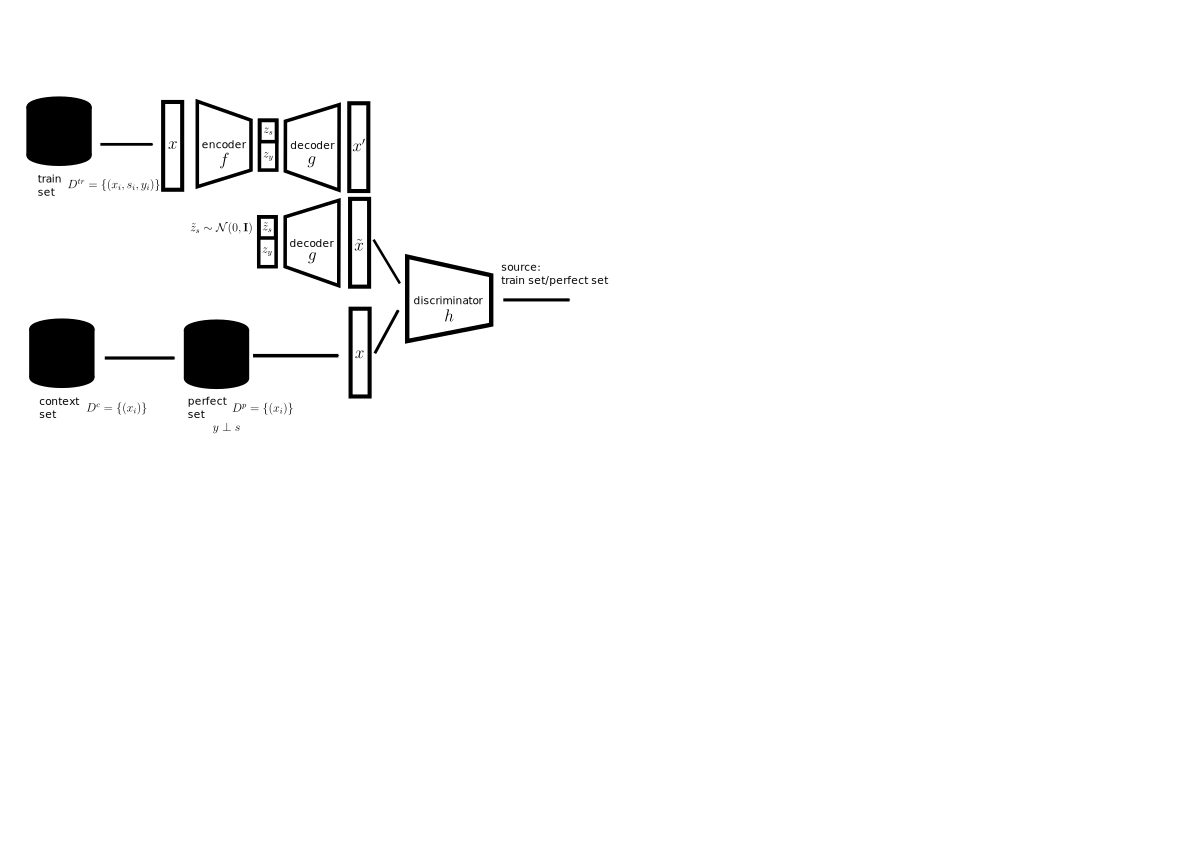
\includegraphics[width=0.9\textwidth]{paper3/figures/SSL-framework}
    % 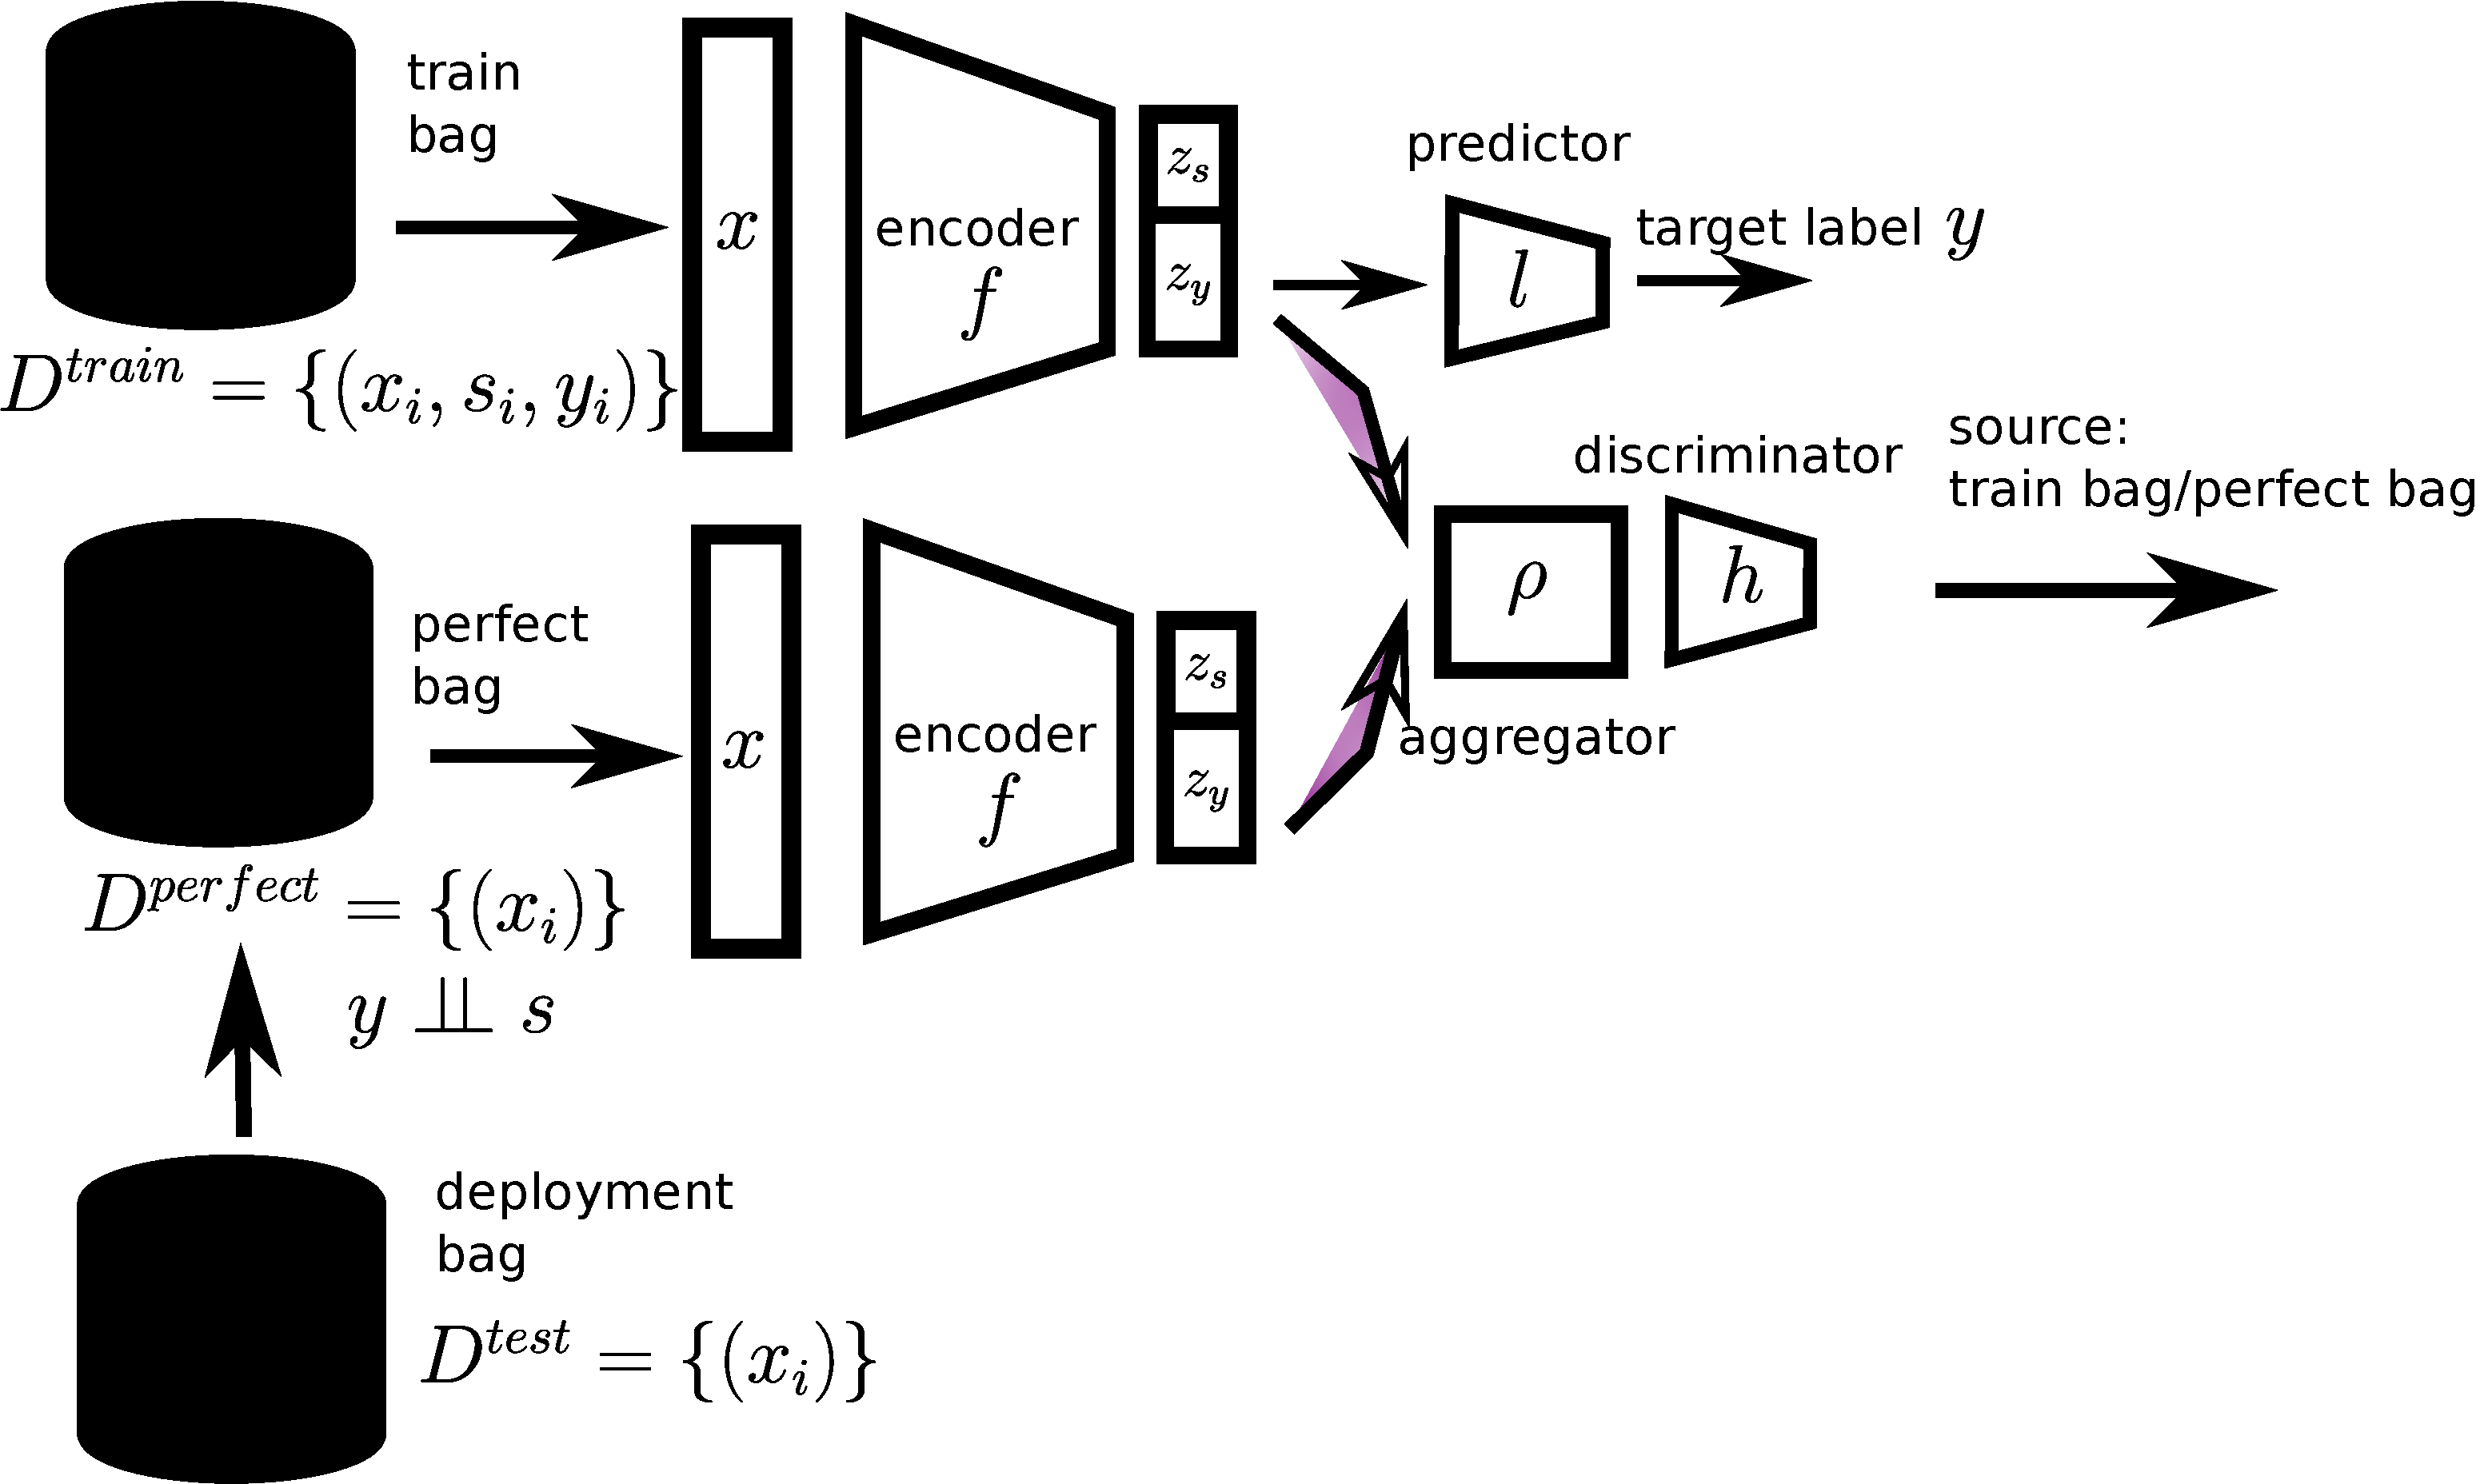
\includegraphics[width=\textwidth]{paper3/figures/SSL-framework-withPred.pdf}
    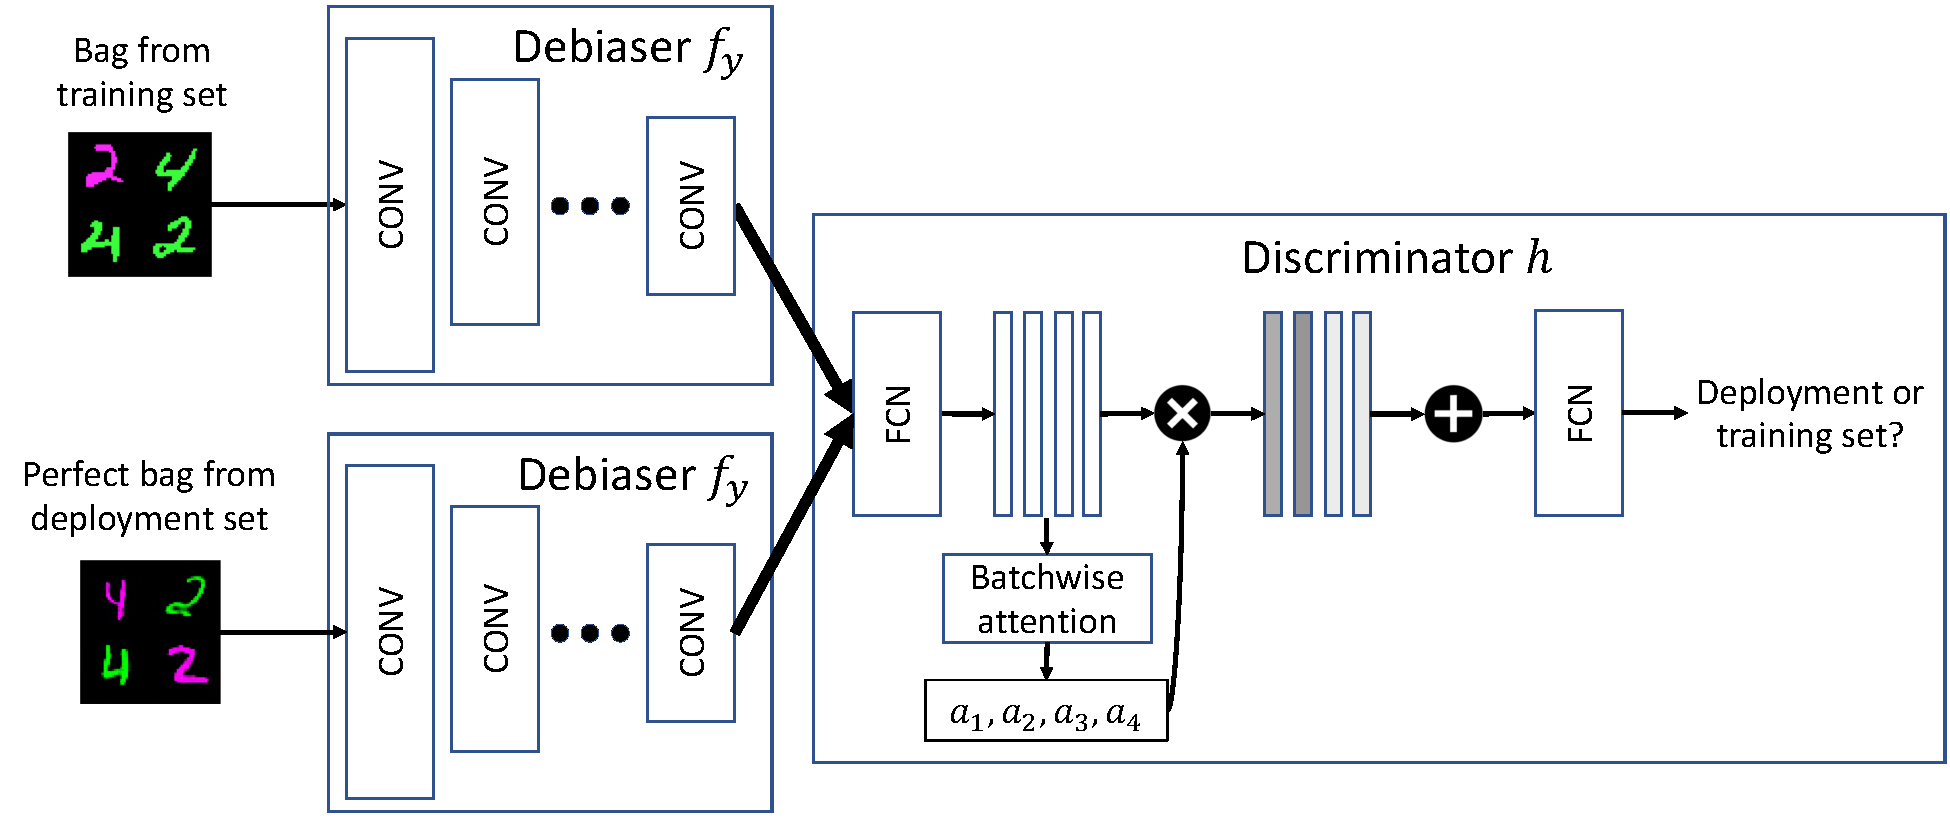
\includegraphics[width=\textwidth]{paper3/figures/zsf_diagram.pdf}
    \caption{%
    The main components involved in our proposed disentangling method, $f_y$ (debiaser) and $h$ (discriminator). The debiaser is trained to produce encodings, $z_y$ of the data that are invariant to the source dataset and thereby the subgroups identifying it. In order to determine whether a bag of encodings originates from the training set or the deployment set, the discriminator performs an attention-weighted aggregation over the bag dimension to model interdependencies between the samples. In the case of Coloured MNIST where {\color{purple}purple} fours constitute the missing subgroup, the discriminator can identify an encoding of a bag from the training set by the absence of such samples so long as colour information is detectable in $z_y$, serving as an error signal for the debiaser.
    }%
    \label{fig:architecture}
\end{figure}%
% \end{figure}
%\end{wrapfigure}
% \hfill
% \begin{figure}
\begin{figure}[t]
    \centering
    % if you want to make changes to the diagram, it is located here:
    % https://drive.google.com/file/d/1M37m4rVj1EGrFJb9QzK32bs8swepiaZ1/view?usp=sharing
    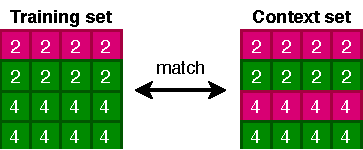
\includegraphics[width=0.5\textwidth]{paper3/figures/fdm.pdf}
    \caption{%
    Illustration of distribution matching.
    In this example, the training set is lacking {\color{purple}purple} 4's.
    By enforcing the subspace $z_y$ to have the same distribution for both the training and deployment set, the model is encouraged to learn a representation that is invariant to colour (or $s$ in general.)
    For this to work, it is crucial that the bags be approximately balanced (perfect bags).
    }%
    \label{fig:matching-diagram}
% \end{subfigure}
% \caption{%
% Overview of the disentangling framework with a perfect (balanced) bag as an inductive bias.
% }%
% \label{fig:framework}
\end{figure}

\section{Methodology}\label{sec:methodology}
\subsection{Theoretical background}
In this section, we first formalise the problem of hidden stratification with zero data (zero-label stratification) and the related issue of algorithmic bias. 
%
We then theoretically motivate the idea of perfect bags for reducing algorithmic bias, and their use as an inductive bias for disentanglement.\\

\noindent\textsc{Zero-label stratification and algorithmic bias.}
% \textsc{Stratification.}
\;\; Let $S$ denote a set of discrete-valued subgroup labels of the associated domains $\gS$.
%
% $S$ can take the values taken by a single subclass label, or, $S = S_1 \times S_2 \times \ldots \times S_p$ with $S_1, \ldots, S_p$ be discrete-valued subclass labels more generally.
%
$X$, with the associated domain $\gX$, represents other attributes of the data. % that may or may not be influenced by subgroup labels $S$.
%
Let $\gY$ denote the space of class labels for a classification task; $\gY = \{0,1\}$ for binary classification or $\gY = \{1,2,\ldots,C_{\text{cls}}\}$ for multi-class classification.
%
For ease of exposition, we assume that we have multiple sources $\Omega$ of samples, one for each combination of class-label $y$ and subgroup-label $s$.
That is, we have:
\begin{align}
\Omega_{y=y',s=s'},\quad\quad\forall y'\in\mathcal{Y},\forall s'\in\mathcal{S},
\end{align}
where, for example, the source $\Omega_{y=0,s=0}$ supplies all data points with class label $y=0$ and subgroup label $s=0$. 
%
As in a standard supervised learning task, we have access to a labelled training set $\gD_{tr} =\{(x_i, s_i, y_i)\}$, that is used to learn a model $M:\gX \rightarrow \gY$. 
$\gD_{tr}$ is composed of several sources, but lacks samples from some of the sources:
\begin{align}
\exists y'\in \gY,\exists s'\in \gS: \gD_{tr}\cap \Omega_{y=y',s=s'} = \varnothing.
\end{align}
For example, we might be missing samples from two sources: $\Omega_{y=0,s=0}$ and $\Omega_{y=1,s=0}$. 
%
In binary classification, this corresponds to no labelled data for the subgroup label $s=0$, a setting we refer to as \emph{missing subgroup} (MS).
%
Other times, we may observe a one-sided (negative) outcome for the subgroup label $s=0$
(\ie, we have $\gD_\mathit{tr} \cap\Omega_{y=1,s=0} = \varnothing$), giving rise to a setting we refer to as \emph{subgroup bias} (SB).

Once the model $M$ is trained, we deploy it to the diverse real-world data.
%
That is, it will encounter data which has overlap with all sources.
% That is, we have a deployment set, $D_{dep} =\{(x_i)\}$ which has overlap with all sources:
% %_{i=1}^{N^t}
% \begin{align}
%             D_{dep}\cap \Omega_{ys} \neq \varnothing\quad\quad\forall y\in\mathcal{Y},\forall s\in\mathcal{S}.
% \end{align}
If the model relies only on the incomplete training set, it is to be expected that the model will misclassify the subgroups with zero training data.
%
The model becomes biased against those subgroups, leading to unexpectedly poor performance when it is deployed.
%
% We will be precise about the adopted mathematical definitions of algorithmic bias.

%Semi-supervised learning \cite{ChaSchZie06} can alleviate the issue of unfairness to the \emph{invisibles} by mixing labelled with unlabelled data, which is usually much cheaper to obtain. 
%
We propose to alleviate the issue of bias against missing subgroups by mixing labelled data with unlabelled data that is usually much cheaper to obtain \citep{ChaSchZie06}. 
%
In this paper, we refer to this set of \emph{unlabelled} data as the
deployment set\footnote{In our experiments, we report accuracy and bias metrics on another independent test set instead of on the unlabelled data that is available at training time.} $\gD_{dep} =\{(x_i)\}$.
%_{i=1}^{N^c}
%
This 
%context 
deployment set has overlap with all sources:
\begin{align}
  \gD_{dep} \cap \Omega_{y=y',s=s'} \neq \varnothing\quad\quad\forall y'\in\gY,\forall s'\in\gS~.
\end{align}
%The deployment set is much like the deployment set: 
Importantly, the deployment set has no information about class labels $y$ or the subgroup labels $s$.

\paragraph{Relation to algorithmic fairness.}
Training set bias also affects what has been termed \emph{algorithmic fairness},
which is commonly expressed in terms of the predicted class $\hat{y}$ of a machine learning model $M$.
We adopt a statistical notion of algorithmic fairness in which outcomes are balanced under certain conditions between groups of data points with different subgroup labels.
% We adopt a statistical notion of algorithmic fairness in which it balances a certain condition between groups of data points with different subgroup labels.
%
% The variable $\hat{y}$ below is the prediction of a machine learning model $M$.
%
Several statistical bias measures have been proposed
% equality of acceptance rate (demographic parity), equality of true positive rates, equality of true negative rate, equality of positive predicted value, equality of negative predicted value
\citep{kamiran2012data,hardt2016equality,zafar2017fairnesstreatment,chouldechova2017fair,RagBarKleLev20}
(shown below for the case where $s$ and $y$ are binary):
\begin{align}
& P(\hat{y}=1|s=0)=P(\hat{y}=1|s=1)\label{eq:AR}\\
& P(\hat{y}=1|s=0,y)=P(\hat{y}=1|s=1,y) \label{eq:TPR} \\
%& P(\hat{y}=0|s=0,y=0)=P(\hat{y}=0|s=1,y=0) %& \text{(equality of true negative rate)} \label{eq:TNR}\\
& P(y=1|s=0,\hat{y})=P(y=1|s=1,\hat{y}) \label{eq:PPV}
%& P(y=0|s=0,\hat{y}=0)=P(y=0|s=1,\hat{y}=0) & \text{(equality of negative predicted value)}\label{eq:NPV}.
\end{align}
(\ref{eq:AR}) is equality of positive rate; (\ref{eq:TPR}) is equality of true positive/negative rate; (\ref{eq:PPV}) is equality of positive/negative predicted value.
Generally, these statistical notions can be expressed in terms of different (conditional) independence statements between the involved random variables \citep{BarHarNar19}:
% $\hat{y}\perp s$ (equality of acceptance rate), $\hat{y}\perp s\ |\ y$ (equality of true positive and true negative rate), and $y\perp s\ |\ \hat{y}$ (equality of positive and negative predicted value).
$\hat{y}\perp s$ (\eqref{eq:AR}), $\hat{y}\perp s\ |\ y$ (\eqref{eq:TPR}), and $y\perp s\ |\ \hat{y}$ (\eqref{eq:PPV}).
If our training set has no positive outcome for the subgroup label $s=0$, i.e. $\Omega_{y=1,s=0} = \varnothing$, the true positive rate for this subgroup will suffer, and therefore we will likely not be able to satisfy, among others, equality of true positive rate.
In the experimental section, we use metrics based on these equalities to quantify how strongly the predictions are affected by the dataset bias.

\paragraph{Perfect bag.}
We call a sampled set for which $y\perp s$ holds, a perfect bag \citep{chouldechova2017fair,kleinberg2016inherent}.
Such sets are also very desirable when training algorithmically fair classifiers
\citep[see the \emph{sampling} method in][]{kamiran2012data}.
%
%If we have access to perfect bags, we could equalise true positive/negative rates (\eqref{eq:TPR}) and also equalise positive/negative predicted values (\eqref{eq:PPV}) for all demographic groups.
%This can be shown by using the sum and product rule of conditional probabilities, e.g. \citet{KanRotZia19}.
%We consider a binary-valued subgroup label, $s\sp{\prime}$ versus $s\sp{\prime\prime}$. 
%For $s\sp{\prime}$, we can compute: 
%$P(y=1|\hat{y}=1,s\sp{\prime})=$
%%\begin{align}
%$\nicefrac{P(\hat{y}=1|y=1,s\sp{\prime})P(y=1|s\sp{\prime})}{\left(A + B\right)}$, with $A = P(\hat{y}=1|y=1,s\sp{\prime})P(y=1|s\sp{\prime})$ and $B = P(\hat{y}=1|y=0,s\sp{\prime})(1-P(y=1|s\sp{\prime}))$.
%%\end{align}
%We can do similarly for $s\sp{\prime\prime}$.
%The conditional probability on the left hand side is 
%a positive predicted value, and this quantity can be expressed in terms of true positive/negative rates and the base (prior) rate, shown on the right hand side. 
%If we have a perfect bag ($y\perp s$ holds, which means equal base rates $P(y=1|s\sp{\prime}) = P(y=1|s\sp{\prime\prime})$), an equality in the true positive/negative rates will give us an equality in the positive/negative predicted values.
%Similarly, with a perfect bag, we can equalise true positive/negative rates (eq. \ref{eq:TPR}) and also positive rates (eq. \ref{eq:AR}) for all demographic groups.
%From the sum probability rule, we have:
%$
%P(\hat{y}=1|s\sp{\prime})
%= P(\hat{y}=1|y=1,s\sp{\prime})P(y=1|s\sp{\prime}) + P(\hat{y}=1|y=0,s\sp{\prime})(1-P(y=1|s\sp{\prime}))
%$ for $s\sp{\prime}$ value, and accordingly for $s\sp{\prime\prime}$ value.
%Here, a positive rate on the left hand side is related to true positive/negative rates and the base (prior) rate as shown on the right hand side. 
%
Ideally, we would like to sample our deployment dataset as perfect bags.
However, the deployment set is unlabelled and is unlikely to be perfect in practice. 
Instead, we pursue learning under zero-label systematic bias as learning disentangled representations with a collection of \emph{approximately} perfect bags (produced with clustering techniques, see section~\ref{sec:implementation}).
We show that the disentangling procedure is robust enough to work with this relaxation, but that performance scales with how well the deployment set is balanced.

\paragraph{Disentangled representation.}
Disentanglement-learning aims to find a factorised representation of a data point $x$ through mapping functions $f_i$ such that $f_i(x)=z_i$ where $z_1,z_2,\ldots,z_p$ are $p$ distinct (independent) factors of variations, which together form $x$.
%
We can formalise this intuitive definition using group and representation theories \citep{HigAmoPfaRacetal18}, or using structural causal models \citep{SutMilSchBau19}.
%
Specifically for this paper, we would like to split the data representation into two factors as $f_y(x)=z_y$ and $f_s(x)=z_s$ where $z_y$ contains factors that are relevant for $y$-prediction and $z_s$ contains factors related to the subgroup label $s$.
%
Since $s$ is correlated with the class label $y$, we need annotations of the undesired nuisance variable $s$ \citep{jaiswal2018unsupervised,JaiWuAbdNat19} to be successful in using disentanglement learning methods for zero-label stratification. %\citet{jaiswal2018unsupervised,JaiWuAbdNat19}.
%
We have some annotations of subgroup label $s$ in the training set $\gD_{tr} =\{(x_i, s_i, y_i)\}$, however, crucially, due to systematic bias, this set is missing certain subgroups.
%
We have all subgroups in the deployment set $\gD_{dep} =\{(x_i)\}$, 
%(also in the deployment set $\Dcal_{tr} =\{(x_i)\}$), 
though, the challenge is that the subgrouping information is unavailable or hidden at the deployment time.
%
In the following section, we show that we can still leverage the 
deployment set for learning the disentangled representations.

\begin{figure}[ht]
    \centering
    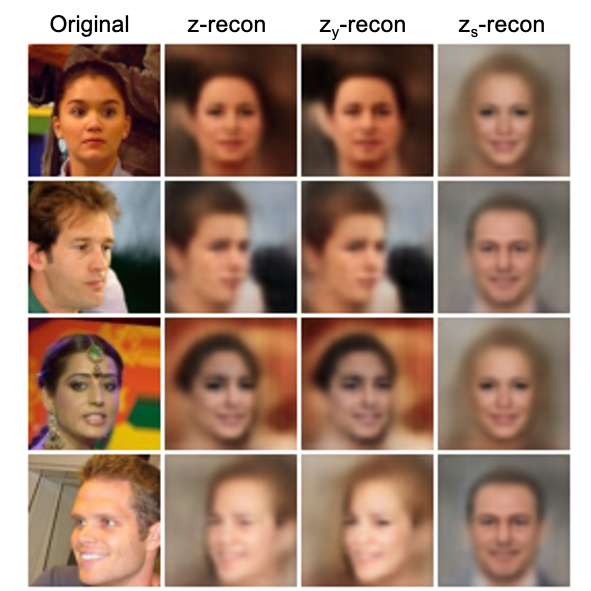
\includegraphics[width=\columnwidth]{paper3/figures/celeba_dep_recon.png}
    \caption{%
    Visualisation of our method's solutions for the CelebA dataset, with``smiling females'' as the missing subgroup.
    Column 1 shows the original images from $x$ from the deployment set of CelebA.
    Column 2 shows plain reconstructions generated from $x_\textit{recon}=g(f_y(x), f_s(x))$.
    Column 3 shows reconstruction with zeroed-out $z_s$: $g(f_y(x), 0)$, which effectively visualises $z_y$.
    Column 4 shows the result of an analogous process where $z_y$ was zeroed out instead.
    }%
    \label{fig:celeba-recons}
\end{figure}

\paragraph{Disentanglement with a collection of perfect bags.}
Our framework for learning the disentangled representations comprises four core modules: 1) \emph{encoder} functions $f_y$ and $f_s$ (which share weights) that embed $x$ into $z_y$ and $z_s$, respectively; 2) a \emph{decoder} function $g$
 that learns the approximate-inverse mapping of $f_y$ and $f_s$: $g: (z_y, z_s) \rightarrow \tilde{x}$ ; 3) \emph{predictor} functions $\ell_y$ and $\ell_s$ that predict $y$ and $s$ from $z_y$ and $z_s$ respectively, and 4) a \emph{discriminator} function $h$ that classifies a given bag of samples embedded in $z_y$ as deriving from the deployment set or the training set; this marks a significant departure from the typical GAN discriminator, which takes as input batches of data and yields a prediction for each sample independently of the other samples in the batch. 
 %
 Fig. \ref{fig:architecture} shows our framework. %, where the training signal comes from the perfect dataset.
 %
 Formally, given bags $\gB_{tr}$ from the training set, and \emph{balanced} (i.e. approximately perfect -- see section \ref{sec:implementation} for details on how this can be practically achieved) bags $\gB_\mathit{perf}$ from the deployment set, we first define, for notational convenience, the loss with respect to the encoder networks, $f_y$ and $f_s$ as
 \begin{align}
     &\,\mathcal{L}_{\text{enc}}(f_y, f_s, h) \nonumber\\
   =&\,\sum_{x \in \mathcal{B}_{tr} \bigcup \gB_\mathit{perf}} L_{\text{recon}} (x,g(f_y(x),f_s(x))) \nonumber\\
     &\,+ \!\!\sum_{x\in \gB_{tr}} \lambda_1 L_{\text{sup}} (y, \ell_y(f_y(x))) + \lambda_2 L_{\text{sup}} (s, \ell_s(f_s(x)))\nonumber\\
     &\,- \lambda_3 (
          \log h(\{f_y(x) | x \in \gB_\mathit{perf}\}) \nonumber\\
         &\quad\quad\,\,\, +  \log h(\{f_y(x) | x \in \mathcal{B}_{tr}\})
     ),
     \label{eq:disentangling}
 \end{align}%
where $L_{\text{recon}}$ and $L_{\text{sup}}$ denote the reconstruction loss, and supervised loss, respectively, and $\lambda_1$, $\lambda_2$ and $\lambda_3$ are positive pre-factors.
The overall objective, encompassing $f_y$, $f_s$, and $h$ can then be formulated in terms of $\mathcal{L}_{\text{enc}}$ as
\begin{align}
    \underset{f_y, f_s}{\textrm{min}}\; \underset{h}{\textrm{max}}\;\mathcal{L}_{\text{total}} = \mathcal{L}_{enc}(f_y, f_s, h)~.
    \label{eq:disentangling_total}
\end{align}%
Aside from being computed over a bag of samples, our adversarial loss differs from that the standard one in that both of its constituent terms are dependent on $f_y$ (the encoder is responsible for producing the ``real'' \emph{and} ``fake'' samples); we allow the gradient to flow through both of these terms, finding that adding a stop-gradient to $\log h(\{f_y(x) | x \in \gB_\mathit{perf}\})$ drastically reduced the convergence-rate and stability of the algorithm.

Eq.~(\ref{eq:disentangling_total}) is computed over batches of bags and the discriminator is trained to map a bag of data points from the training set and the deployment set to a binary label:
$1$ if the bag is judged to have been sampled from the deployment set, $0$ if from the training set.
% Its goal is to effectively estimate the probability that a bag of samples has been sampled from one distribution or the other.
Since the task is a set-classification one, we require that the function it defines respects the exchangeability of the bag dimension -- that is, the discriminator's predictions should take into account dependencies between samples in a bag but should be invariant to the order in which they appear,
\ie\ we have
\(h(\{f_y(x_i)\}^\gB_{b=i}) = h(\{f_y(x_i)\}^\gB_{b=\pi (i)})\)
for all permutations $\pi$.
To make the entirety of the function $h$ -- composed of sub-functions $h_1(h_2(h_3...)))$ -- have this property, requires only the innermost, sub-function, $\rho$ in the chain to have it.
While there are a number of choices when it comes to defining $\rho$, we choose a weighted average $\rho = \frac{1}{\gB} \sum_i(\{\mathrm{attention}(f_y(x_i))\}^\gB_{b=i})$, with weights computed according to a learned attention mechanism. The idea of using an attention mechanism for set-wise classification has been previously successfully explored by \citet{ilse2018attention} and  \citet{lee2019set};
we use the gated attention mechanism proposed by \citet{ilse2018attention} in the experiments, but also tried out the scaled dot-product attention per \citet{vaswani2017attention}, as the bag-wise pooling layer of our discriminator.
% For the latter, we had success defining K and V to be  $z_y$, and Q to be the mean of $z_y$ over $\mathcal{B}$.
% , weighting values (V) according to the similarity between the associated key (K) and query (Q) matrices, as measured by their dot-product. 
% Q, K, and V are not used directly but are first embedded into linear subspaces by matrix-multiplication with learned weight matrices of dimension $\mathbb{R}^{m\times d}$. 
% Q, K, and V are used after they have been embedded into linear subspaces by matrix-multiplication with learned weight matrices of dimension $\mathbb{R}^{m\times d}$. 
The result of $\rho$ is then processed by a series of fully-connected layers, following the DeepSets  \citep{zaheer2017deep} paradigm, which ultimately computes a single prediction for a given bag of samples.

Our goal is that $z_y$ is invariant to the subgroup $s$.
However, what the adversarial loss actually enforces is the $z_y$ has the same distribution for the bags from the deployment set and the bags from the training set.
To ensure that the network learns the correct task,
it is crucial that subgroup membership is the only differing factor between the two types of bags.
The first step towards this goal is that bags from the deployment set are balanced (or \emph{perfect}):
all combinations of $s$ and $y$ appear at the same rate.
The second step is that, in the bags from the training set, the possible values of $y$ have to appear at the same rate,
because $y$ is meant to be preserved;
thus, $P(y_\mathit{tr}=0)=P(y_\mathit{tr}=1)=\mathellipsis$.
Finally, within the classes, subgroups should appear at equal rate:
$P(s_\mathit{tr}=0|y_\mathit{tr}=y')=P(s_\mathit{tr}=1|y_\mathit{tr}=y')=\mathellipsis$.
For example, if the bag size is 4, $Y$ and $S$ are binary, and the combination $(y=1,s=0)$ is missing,
then each bag should contain 2 samples of $(y=1,s=1)$ and 1 sample each of $(y=0,s=0)$ and $(y=0,s=1)$
(see also fig.~\ref{fig:matching-diagram}).
This ensures that the bags from the training set only differ in those samples from the deployment bags,
where a subgroup is missing.
%
% We know that the $y\perp s$ condition holds in the perfect bag, but not in the training set due to sampling bias.
% To do well, the discriminator should rely on this knowledge.
% More concretely, since the deployment and training set have differing support over $\Scal \times \Ycal$, namely $(\Scal_{tr} \times Y_{tr}) \subsetneq (\Scal_\mathit{perf} \times \Ycal_\mathit{perf})$, that support serves as an indicator of the distribution from which the data has been drawn.
% The scenarios we consider dictate $\Ycal_{tr} = \Ycal_\mathit{perf}$, making the disentangling well-posed.
% However, since we wish to use $\Scal_{dep} \times \Ycal_{dep} \setminus \Scal_{tr} \times \Ycal_{tr}$ as the training signal for the encoder, and not the relative frequency of the target classes,
% it is important that, like the deployment set, we weight the samples of the training set such that both $P(y_{tr})$ and $P(s_{tr}|y_{tr})$ are equal for all $s_{tr}, y_{tr} \in \Scal_{tr} \times \Ycal_{tr}$.
To guide the network towards the desired solution, we supplement this implicit constraint with the explicit constraint that $z_y$ be predictive of $y$, which we achieve using a linear predictor $l$. Whenever we have $\textrm{dim}(\mathcal{S}) > 1$ %(in our experiments this corresponds to the \emph{subgroup bias} setting)
we can also impose the same constraint on $z_s$, but with respect to $s$.
With these conditions met, to fool the discriminator,
the encoder must separate out information pertaining to $S$ into the space $z_s$ not part of the discriminator's input,
leaving only subgroup-unrelated information in $z_y$.

%We note that there remains the potential for one degenerate solution, namely that $f_s$ could encode information pertaining to $s$ \emph{and} $y$ in $z_s$, \ie\ the section of the latent space not input to the discriminator.
%In this situation, $z_y$ simply contains residual information that cannot be used to distinguish the deployment from the training set.
%To minimise the risk of this solution, we restrict the amount of information that can be encoded in $z_s$ by setting its dimensionality equal to $\ceil{\text{log}_2(\text{dim}(\mathcal{S}))}$;
%\eg, in the case of binary $s$, we restrict $z_s$ to be one-dimensional.
%Additionally, $z_s$ can be discretised with a straight-through estimator for the gradient \cite{bengio2013estimating}.
%
In the \emph{missing subgroup} scenario, the disentangling supervision is weaker.
Thus, for this case, we restrict the amount of information that can be encoded in $z_s$ by setting its dimensionality equal to $\ceil{\text{log}_2(\text{dim}(\mathcal{S}))}$;
\eg, in the case of binary $s$, we restrict $z_s$ to be one-dimensional.
Additionally, $z_s$ can be discretised with a straight-through estimator of the gradient \citep{bengio2013estimating}.

Note that as long as the model sees the different \(s\)-\(y\)-combinations at the right proportions,
disentangling can (to an extent) also be achieved without the bag-wise loss
(\ie, when the bag size is set to 1).
The model then has to learn an implicit prior for which \(s\)-\(y\)-combinations to expect
in the two different sets -- training set and deployment set.
However, in our preliminary experiments we found this sample-wise approach to work much poorer
than using a bag-wise loss.
For those experiments, the batch was balanced in the same way as described above for the bags,
but the batch was not subdivided into bags
and there was no attention or aggregation method applied to the batch:
the loss was just computed per sample.
From the poor performance,
we inferred that the sample-wise loss lacks the necessary context
to easily differentiate between the two datasets.

Our contribution to the disentanglement problem is thus two-fold:
i) the use of the difference between two distinct sets as the supervision signal,
and ii) the use of a bag-wise loss
(where the bags are sampled to represent their corresponding data distribution in an idealised way)
which allows the model to contrast the two sets more easily.
Together, they form the idea of disentangling with ``perfect bags''.

As mentioned in \secref{ssec:on-disentangled-representation-learning},
\citet{locatello2020weakly} learned to disentangle from non-i.i.d.\ pairs
which share at least one underlying factor.
In our scenario, constructing the pairs each out of one sample from the training set and one sample from the deployment set
would satisfy this requirement if we allow the `underlying factor' to be quite abstract
(see also the section below for a discussion of this).
However, constructing the pairs each out of two \emph{bags} instead of two samples
makes the analysis much clearer:
bags from the training and deployment set are constructed such
that they both have the same distribution of \(y\) values (a uniform distribution over \(y\)),
but they differ in the distribution of \(s\) values.
Thus, the \emph{shared} factor is the one concerning the prediction target \(y\),
and the \emph{differing} factor is the one concerning \(s\).

\paragraph{Disentanglement guarantees.}
%\citet{ShuCheKumErmetal20} decomposed disentanglement into two distinct concepts: consistency and restrictiveness.
%
%The decomposition allows for correlated factors of variations, which is crucial in our case as the subgroup label $s$ is correlated with the class label $y$. 
%
%We now provide a single-factor disentanglement guarantee of our disentanglement with a collection of perfect bags approach based on theoretical results of \citet{ShuCheKumErmetal20}.
%
Under \citet{ShuCheKumErmetal20}'s framework, our disentanglement supervision corresponds to \emph{match pairing}:
We observe samples from a pair of distributions (deployment set and training set).
As an example, we consider coloured MNIST with two classes (digits 2 and 4) and two subgroups (colours purple and green), where the training set is lacking the combination of digit 4 and colour purple.
Sample pairs from the two distributions have a shared underlying factor: 2's can be purple and green.
The pairs also have a factor that differs: in the training set, a 4 can only be green; in the deployment set, it can have both colours.
Theorem 1 in \citep{ShuCheKumErmetal20} guarantees then that a (sufficiently powerful) disentangling encoder will produce a disentangling that is \emph{consistent} with respect to the shared factor and \emph{restricted} with respect to the changing factor.
In our case, $z_y$ will capture the shared factor and $z_s$ the changing factor.
For the invariant representation, we drop $z_s$, which can be seen as setting this value to 0; as $z_s$ has guaranteed \emph{restrictiveness}, the effect of changing $z_s$ is restricted to changing the corresponding factor,
which in the example refers to whether or not 4's can be purple.
%We show that this is in fact the case for our approach, and we focus on the $z_s$ factor for the explanation.
%
%Share pairing is where $z_s$ is the only factor that is shared between training bags and perfect bags\footnote{We focus on groups of data points in contrast to the paired setting in \citet{ShuCheKumErmetal20}.}. 
%
%Change pairing is where $z_s$ is the only factor that is changed.
%

% \textbf{Connection with the ``we're all equal'' worldview.}
% Why do we substitute $z_s$ with a random vector ($\tilde{z}_s$) to make our training set to be similar to the perfect set? 
% %
% This substitution procedure actually aligns with the view that various subgroup labels such as race and gender are not entangled with a person's intelligence, grit and consequently those subgroup labels have no bearing on ground truth class labels, such as performing well on the job, that might be functions of these qualities \cite{FriSchVen16}. 
% %
% If our disentangled representation produces the same label distributions regardless on the values of $z_s$, then we know that we have reached the property of a perfect dataset.
% %%%comment out:
% On a practical side, substituting $z_s$ with a random vector masks out the information about the protected group. This prevents the discriminator from learning a shortcut that samples from invisible demographics are coming from the perfect set only. 

% \textbf{How do the $z_y$ and $z_s$ partitions acquire their semantics?}
% To achieve disentanglement,
% we use the adversary to encourage the model to make the distribution $z_y$
% the same for both the training set and the deployment set.
% However, there are multiple ways to achieve this.
% One is to sort all information about $s$ into what we call $z_y$ and information about $y$ into what we call $z_s$.
% In order to prevent such solutions,
% $z_y$ is encouraged to contain information about $y$ via a classifier that predicts $y$ from $z_y$.
% For the same reason, we predict $s$ from $z_s$ during training.
% This is possible because we have access to the $y$ and $s$ labels from the \emph{training} set.
% On their own, these labels are not enough to fully disentangle the inputs,
% either because $s$ and $y$ are highly correlated in the training set,
% or because the training sets lacks samples for a certain $s$ value entirely,
% but they are still valuable in constraining the model to find the right solution.

% Another way in which we ensure that $s$ and $y$ are sorted correctly
% is by balancing the batches from the deployment set:
% this ensures that $s$ and $y$ are (at least approximately) independent.

% Note furthermore that the task of sorting information into $z_y$ and $z_s$ is orthogonal to the task of the reconstruction loss in the autoencoder.
% So, there is no trade-off to balance the autoencoder loss against discriminator loss, since the discriminator is only privy to the $z_y$ information while the autoencoder has both $z_y$ and $z_s$ available for the reconstruction.

% \textbf{Ablations.}
% We train an adversarial network for our disentangling strategy to learn how to distinguish between the training set and the perfect set. 
% %
% This adversarial network is analogous to discriminators in generative adversarial networks (GANs) \cite{GooAbaMirXuetal14} where their role is to discriminate between fake and real images created by the generator. %
% We can therefore conduct similar equilibrium analysis as the traditional generative adversarial network model.
% %
% We know that the adversarial formulation in eq. (\ref{eq:disentangling}) has a global optimum for $p(g(\tilde{z}_s:=\mathcal{N}(0,\mathbf{I}),z_y))_{\text{training set}} = p(x)_{\text{perfect set}}$.
% %
\begin{figure*}[ht]
  \centering
  \includegraphics[width=\columnwidth]{paper3/figures/cmnist_2v4_partial_acc.pdf}
  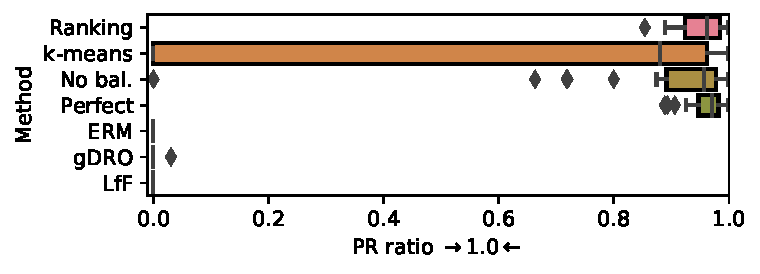
\includegraphics[width=\columnwidth]{paper3/figures/cmnist_2v4_partial_prr.pdf}
%   \includegraphics[width=\columnwidth]{paper3/figures/cmnist_2v4_partial_tpr.pdf}
%   \includegraphics[width=\columnwidth]{paper3/figures/cmnist_2v4_partial_tnr.pdf}
  \caption{
    Results from 30 repeats for the Coloured MNIST dataset with two digits, 2 and 4, with \emph{subgroup bias} for the colour `{\color{purple}purple}': for {\color{purple}purple}, only the digit class `2' is present.
    \textsc{Left}: Accuracy.
    \textsc{Right}: Positive rate ratio.
    % \textbf{Bottom left}: True positive rate ratio.
    % \textbf{Bottom right}: True negative rate ratio.
    For the \texttt{Ranking} clustering, the clustering accuracy was 96\% $\pm$ 6\%;
    for \texttt{K-means} it was 64\% $\pm$ 10\%.
  }%
  \label{fig:cmnist-2v4-partial}
\end{figure*}
\begin{figure*}[ht]
  \centering
  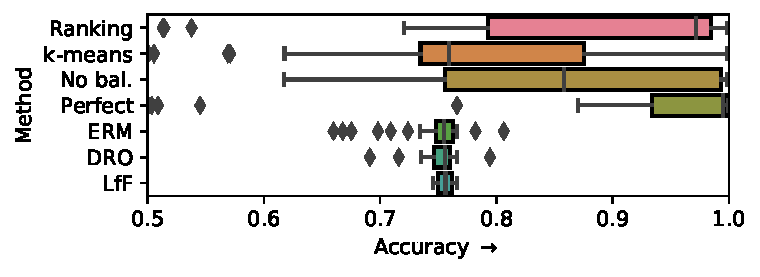
\includegraphics[width=\columnwidth]{paper3/figures/cmnist_2v4_miss_s_acc.pdf}
  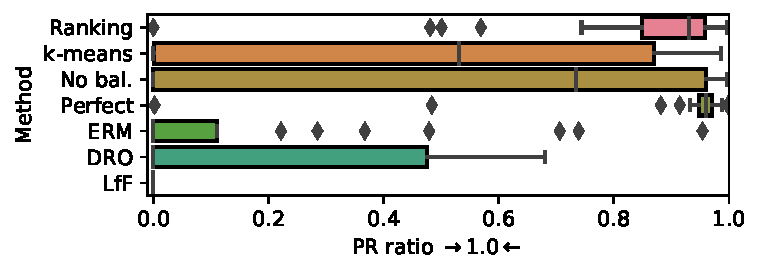
\includegraphics[width=\columnwidth]{paper3/figures/cmnist_2v4_miss_s_prr.pdf}
%   \includegraphics[width=\columnwidth]{paper3/figures/cmnist_2v4_miss_s_alt_tpr.pdf}
%   \includegraphics[width=\columnwidth]{paper3/figures/cmnist_2v4_miss_s_alt_tnr.pdf}
  \caption{
    Results from 30 repeats for the Coloured MNIST dataset with two digits, 2 and 4, with a \emph{missing subgroup}: the training dataset only has {\color{green}green} digits.
    \textsc{Left}: Accuracy.
    \textsc{Right}: Positive rate ratio.
    % \textbf{Bottom left}: True positive rate ratio.
    % \textbf{Bottom right}: True negative rate ratio.
    For the \texttt{Ranking} clustering, the clustering accuracy was 88\% $\pm$ 5\%;
    for \texttt{K-means} it was 72\% $\pm$ 16\%.
  }%
  \label{fig:cmnist-2v4-miss-s}
\end{figure*}
\begin{figure*}[ht]
  \centering
  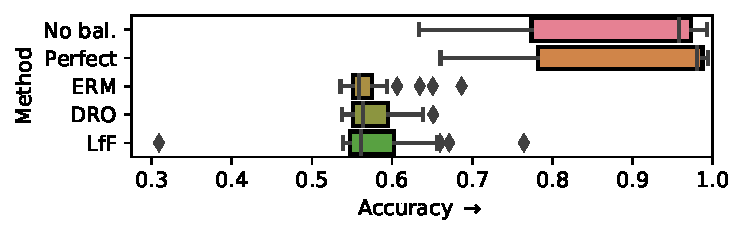
\includegraphics[width=\columnwidth]{paper3/figures/cmnist_3dig_4miss_acc.pdf}
  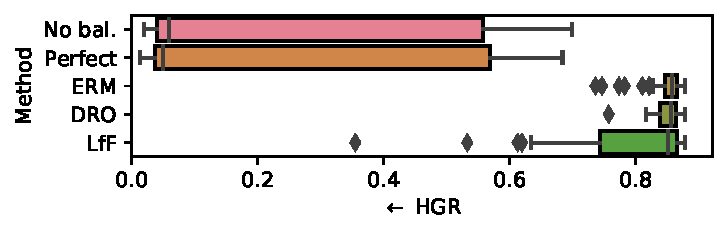
\includegraphics[width=\columnwidth]{paper3/figures/cmnist_3dig_4miss_hgr.pdf}
%   \includegraphics[width=\columnwidth]{paper3/figures/cmnist_3dig_4miss_pr.pdf}
%   \includegraphics[width=\columnwidth]{paper3/figures/cmnist_3dig_4miss_tpr.pdf}
%   \includegraphics[width=\columnwidth]{paper3/figures/cmnist_3dig_4miss_tnr.pdf}
  \caption{
    Results from 30 repeats for the Coloured MNIST dataset with three digits: `2', `4' and `6'.
    Four combinations of digit and colour are missing: {\color{green}green} 2's, {\color{blue}blue} 2's, {\color{blue}blue} 4's and {\color{green}green} 6's.
    \textsc{Left}: Accuracy.
    \textsc{Right}: Hirschfeld-Gebelein-R\'enyi maximal correlation \citep{renyi1959measures} between $S$ and $Y$.
    % \textbf{Right}: Positive rate ratio.
    % \textbf{Bottom left}: True positive rate ratio.
    % \textbf{Bottom right}: True negative rate ratio.
  }%
  \label{fig:cmnist-3dig-4miss}
\end{figure*}
\begin{figure*}[ht]
  \centering
  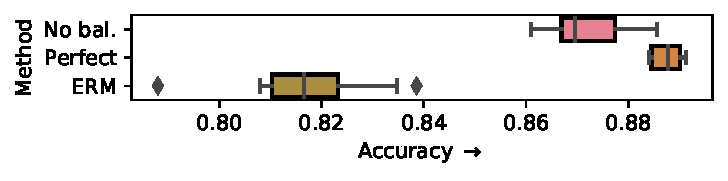
\includegraphics[width=\columnwidth]{paper3/figures/celeba_gender_smiling_acc.pdf}
  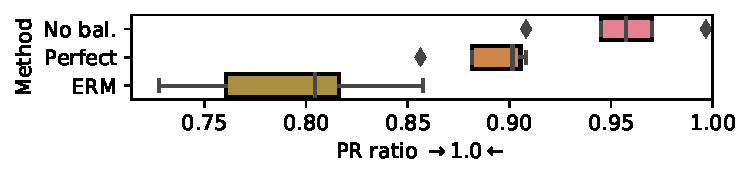
\includegraphics[width=\columnwidth]{paper3/figures/celeba_gender_smiling_prr.pdf}
%   \includegraphics[width=\columnwidth]{paper3/figures/celeba_gender_smiling_tpr.pdf}
%   \includegraphics[width=\columnwidth]{paper3/figures/celeba_gender_smiling_tnr.pdf}
  \caption{
    Results from 10 repeats for the CelebA dataset with the \emph{subgroup bias} setting.
    The task is to predict ``smiling'' vs ``non-smiling'' and the subgroups are based on gender.
    The subgroup ``female'' is missing samples for the ``smiling'' class.
    \textsc{Left}: Accuracy.
    \textsc{Right}: Positive rate ratio.
    % \textbf{Bottom left}: True positive rate ratio.
    % \textbf{Bottom right}: True negative rate ratio.
  }%
  \label{fig:celeba-gender-smiling}
\end{figure*}

\subsection{Implementation}
\label{sec:implementation}
Our proposed framework, demonstrated in fig.\,\ref{fig:architecture}, entails two steps: 1) sample perfect bags from an unlabelled deployment set, and 2) produce disentangled representations using perfect bags for adversarial distribution-matching.

\paragraph{Constructing approximately perfect bags via clustering.}
We cluster the data points from the deployment set into $K=\textrm{dim}(\mathcal{Y})\cdot \textrm{dim}(\mathcal{S})$ number of clusters, i.e. the number of data sources $\Omega_{y,s}$. 
%, using a learned embedding $z$.
%
We use the k-means clustering algorithm, and a recently proposed method based on rank statistics \citep{HanRebEhrVedetal20}.
%
The cluster assignments can then be used to evenly stratify the deployment set into perfect batches, to be used by the subsequent disentangling phase.
%
% The objective for clustering can be written as a binary cross-entropy loss, induced by the following binary classification problem -- for any two data points in the deployment set to decide whether or not they belong to the same cluster:
% %
% \begin{align}
%  \mathcal{L}_{\textit{unsup}} &= -\frac{1}{N^2}\sum_{i,j} [s_{ij}\: \text{log} (C(z_i)^\top C(z_j)) \nonumber\\
%  &+ (1-s_{ij}) \: \text{log}(1-C(z_i)^\top C(z_j))].
%  \label{eq:clustering}
%  \end{align}
% %
% Here, $N^2$ is the amount of sample pairs,  $s_{ij}$ are binary labels capturing that similar data points belong to the same group, $s_{ij}=1$, while dissimilar ones do not, $s_{ij}=0$. 
% %
% Since the deployment set is unlabelled, $s_{ij}$ are unknown. 
% %
% We estimate $s_{ij}$ with the robust rank statistics approach (described below) and use the estimates as pseudo-labels in \eqref{eq:clustering}. 
% %
% The dot-product $C(z_i)^\top C(z_j)$ measures the similarity of the two data points $z_i$ and $z_j$ to score whether they share a cluster.
% %
% This is computed on the embedding of the softmax classifier $C: \mathcal{Z} \rightarrow \{1,\ldots, K\}$. 
% %
% In addition to this unsupervised training, the classifier $C$ is also trained on the labelled data using the standard cross-entropy loss.  
% %We train the classifier $C$ on the training data using a standard cross-entropy loss and the labelled sources $\Omega_{y,s}$. 
% %
% This way, the data points in the deployment set that are similar to the known demographics are assigned to the associated clusters, while the dissimilar data points form the new clusters corresponding to the invisible groups. 

% The method of rank statistics \citep{YagStrRosLin11,DeaRuzSegShletal13,HanRebEhrVedetal20} avoids comparing the vectors $z_i$ and $z_j$ directly, and instead ranks the values in $z_i$ and in $z_j$ by their magnitudes, and compares the top-$U$ rankings (we found $U = 5$ to perform well in our experiments).
% %
% If the rankings obtained for two unlabelled data points $z_i$ and $z_j$ are the same, they are assigned to the same class, $s_{ij}=1$. 
% %
As a result of clustering, the data points in the deployment set $\gD_\mathit{dep}$ are labelled with cluster assignments 
$\gD_\mathit{dep}=\{(x_i, c_i)\}$, $c_i = C(z_i)$.
%
We balance $\gD_\mathit{dep}$ so that all clusters have equal size to form a perfect bag
% (see fig. \ref{fig:teaser})
, and use it as a supervision signal for the disentangling step.
%
%Note that our method of constructing the perfect dataset based on clustering does not require solving the linear assignment problem of cluster-source association. This is particularly suitable for exploring the setting where invisible demographics are formed of multiple sources.

% \textbf{Is an \emph{explicit} identification of all clusters, i.e. which demographic groups and labels they correspond to, required?}
\paragraph{Clustering requirements.}
For constructing the perfect bags, the correspondence between the clusters and the class-labels/subgroup-label pairs does not need to be known.
The clustering is only needed for drawing an equal number of samples from each cluster for each bag of samples.
% Constructing the bags in this way does \emph{not} require us to solve linear assignment problem of cluster-source association.
%% (Thomas doesn't understand this sentence:)
% This is particularly advantageous for exploring the setting where invisible demographics are formed of multiple sources.
In our experiments, we provide an analysis with unsupervised k-means clustering where we do not use annotations from the training set as side information, even for the \emph{known} groups. 
When clustering with the training labels (such as with the rank statistics approach), we use the information that they provide to ensure samples from the \emph{known} subgroups are clustered together with others with the same label.

\paragraph{Clustering guarantees.}
By leveraging the feature space of deep models, previous research has shown that semantically meaningful clusters can be discovered without the need for ground-truth annotations
\citep[for example][]{RayDunCarRe20,GanVanGeoProetal20,SohDunAngGuetal20,HanRebEhrVedetal20}.
\citet{SohDunAngGuetal20} recently provided a ``clustering guarantee'' when assuming access to ground truth class labels $y$ and using clustering within each class to generate approximate subgroups $s$.  
%
Even with infinite data, accurate identification of the subgroups is unfortunately impossible. 
%
Instead, \citet{SohDunAngGuetal20} showed that the error in their quantity of interest, classification loss for each subgroup, can be bounded by the total variation estimation error in the mixture-of-Gaussians case.   
%
Our primary goal is to ensure good construction of perfect bags.
We can adapt the analysis of \citet{SohDunAngGuetal20} to bound the error of our quantity of interest, \emph{aggregate statistics} of the approximated perfect bag for each subgroup.
%
We can subsequently apply the union bound to take into account that we have a fully-unlabelled setting.


\subsection{Limitation and intended use}
\label{sec:limitations}
% First, dataset consumers should take extra care about the cost-benefit analysis of selecting particular datasets for their machine learning tasks. 
%
Although having zero labelled examples for some subgroups is not uncommon due to the effects of systematic bias,
we should make a value-judgement on the efficacy of the dataset with respect to a task.
%
% {\color{red}Corrective action such as the one described in this paper or inaction should be recorded.}
We can then decide whether or not to take corrective action as described in this paper.

A limitation of the presented approach is that, for constructing the perfect bags used to train the disentangling algorithm, we have relied on knowing the number of clusters \emph{a priori}, something that, in practice, is perhaps not the case. 
%
Removing this dependency through automatic determination of the number of clusters would generalise our method further but this line of research is challenging and extends beyond the scope of the current paper. 
%
One difficulty is that we need to ensure that the small but salient clusters are correctly identified. 
%
% In the case of 2-digit Coloured MNIST, for example, the deployment set may contain only a small portion of {\color{purple}purple} fours relative to the other subgroups, meaning that the cluster they form can be easily overlooked by a clustering algorithm in favour of larger but less salient clusters (which may be sub-clusters of other digit/colour combinations). 
The cluster formed by an underrepresented subgroup can be easily overlooked by a clustering algorithm in favour of larger but less salient clusters
(which may be sub-clusters of other, larger, subgroups). 

% By leveraging feature space of deep models, previous research has shown that semantically meaningful clusters can be discovered without the need for ground-truth annotations
% (for example \citet{RayDunCarRe20,GanVanGeoProetal20,SohDunAngGuetal20,HanRebEhrVedetal20}), but how useful these annotations are in practice is still up for question.

% In this paper, we aim to highlight the problem of zero-label stratification that can result from systematic bias, and to make a case for it as something to be seriously considered (even if to be dismissed) when planning, building, evaluating and regulating machine learning systems.
%Clearly, the use of algorithmic approaches still requires human review in a manner that is similar to error auditing, but is less dependent on the specific human auditor to initially identify the stratification. While algorithmic approaches to measurement can reduce burden on human analysts and take advantage of learned encodings to identify subclasses, their efficacy is limited by the difficulty of separating important subclasses in the feature space analysed.

\section{Experiments}
We perform experiments using image and tabular datasets: Coloured MNIST \citep{kim2019learning}, CelebA \citep{liu2015faceattributes} and Adult Income\footnote{{Results for Adult Income dataset and discussion can be found in the supplementary material.}} \citep{Dua:2017} that are publicly available. 
%arjovsky2019invariant, KehBarThoQua20
%
To validate the first step of creating the perfect bags, we compare the performance of our disentangling model when paired with each of four different balancing methods:
1) with clustering via rank statistics (\texttt{Ranking});
2) with clustering via k-means (\texttt{K-means}); 
3) without balancing, when the deployment set $\gD_{dep}$ is used as is (\texttt{No bal.});
4) with balancing done using the ground-truth class and subgroup labels (\texttt{Perfect}) that would in practice be unobservable; this provides insight into what can be achieved under ideal conditions and how sensitive the method is to imperfections in the bag-balancing.
 
To validate the disentangling step, we compare with three other baselines.
In all cases, the training set is balanced in the same fashion required for our method.
This is similar in effect to the sampling method proposed by \citet{kamiran2012data} but with those samples with the same class label as the missing sources upsampled, based on knowledge of $\text{dim}(\mathcal{S})$.
We denote a classifier trained with cross-entropy loss on this data as \texttt{ERM}.
The second of the aforementioned baselines is \texttt{DRO} \citep{HasSriNamLia18}, which functions without subgroup labels by minimising the worst-case training loss over all possible groups that are above a certain minimum size;
along with a variant of it, \texttt{gDRO} \citep{sagawa2019distributionally}, that exploits subgroup label information but is then only applicable when $\text{dim}(\mathcal{S}_{tr}) > 1$.
Third, we have the \texttt{LfF} model proposed by \citet{nam2020learning} that works by reweighting the cross-entropy loss of a classifier using the predictions of a purposely biased sister network.

%
%%%%%OR
%During training, the {\color{green}green} colour group is observed in both digits (sources $\Omega_{y=\text{'two' }s=\color{green}green}$ and $\Omega_{y=\text{'four' }s=\color{green}green}$), but for the {\color{purple}purple} colour group, we only observe the one-sided outcome ($\Omega_{y=\text{'two'}s=\color{purple}purple}$), so the source $\Omega_{y=\text{'four'}s=\color{green}green}$ defines invisible demographic.  
%
\subsection{Coloured MNIST}
The MNIST dataset \citep{lecun1998gradient} consists of 70,000 (60,000 designated for training, 10,000 for testing) images of grey-scale hand-written digits. We colour the digits following a similar procedure to that outlined by \citep{kim2019learning}, randomly assigning each sample one of ten distinct RGB colours. Each source is then a combination of digit-class (class label) and colour (subgroup label). We use no data-augmentation aside from symmetrically zero-padding the images to be of size 32x32.
We create imbalance in both $D_{dep}$ and $D_{tr}$ by sub-sampling the remaining sources;
we do this to render a more realistic setting in which the deployment set is not innately balanced and demands preliminary clustering to construct approximately perfect bags. The sub-sampling proportions used for each set of experiments can be found in the appendix.

We begin by considering a binary, 2-digit, 2-colour, variant of the dataset with $Y = \{2, 4\}$ and $S = \{\text{\color{green}green}, \text{\color{purple}purple}\}$.
For this variant we explore both the SB (subgroup bias) and MS (missing subgroup) settings.
To simulate the SB setting, we set  $\Omega_{y=4,s=\text{\color{purple}{purple}}}$ to be the missing source.
To simulate the MS setting, where we have training data for only a single subgroup, we set both $\Omega_{y=\text{'two'},s=\color{purple}purple}$ and $\Omega_{y=\text{'four'},s=\color{purple}purple}$ to be the missing sources (i.e. $D_{tr}$ consists of only $\text{\color{green}{green}}$ digits).
%

Fig.~\ref{fig:cmnist-2v4-partial} shows the results for the SB setting. We see that the performance of our method directly correlates with how balanced the bags are, with the ranking of the different clustering methods being \texttt{Perfect} $>$ \texttt{Ranking} $>$ \texttt{No bal.} $>$ \texttt{K-means}. Even without balancing (\texttt{No bal.}) our method greatly outperforms the baselines methods, which all exhibit similar performance to one another in terms of both accuracy and PR ratio (positive rate ratio).
The PR ratio is given by $\nicefrac{P(\hat{y}=1|s=1)}{P(\hat{y}=1|s=0)}$;
it quantifies how invariant the classifier output $\hat{y}$ is to the subgroups.
The optimal value is 1.
% The PR ratio being ${\approx} 0$ indicates these methods degenerate to predicting positive for only a single class, a failure case our method avoids.

Fig.~\ref{fig:cmnist-2v4-miss-s} shows that the problem of \emph{missing subgroups} is harder to solve.
Again we see that poor clustering (in the case of \texttt{K-means}) is detrimental to the disentangling procedure, though for all balancing strategies the IQR is significantly higher than observed in the MS setting, along with there being a number of extreme outliers. The median, however, remains high, which is reflective of the ``hit-or-miss'' performance of the method under these conditions, but where the number of hits far outweighs the number of misses. Visualisation of the reconstructions with $z_y$ zeroed-out suggest that misses often mostly occurred due to the semantic information being concentrated in $z_s$ while $z_y$ is left to contain only residual information, even when $z_s$ was set to be one-dimensional and binarised. We leave it to future work to explore how to better offset such degeneracies.

To investigate how an increase in the number of classes affects disentangling of classes and groups, we look to a 3-digit, 3-colour variant of the dataset in the SB setting where four sources are missing from $D_{tr}$.
Results for this configuration are shown in fig.~\ref{fig:cmnist-3dig-4miss}.
We see that the performance of \texttt{No bal.} is quite close to that of \texttt{Perfect}, we suspect this is because balancing is less critical with the increased number of subgroups strengthening the training signal.
As the PR ratio is not a suitable metric for non-binary $S$,
we instead quantify the invariance of the predictions to the subgroup with
the HGR maximal correlation \citep{renyi1959measures}.
 
\subsection{CelebA}
To demonstrate our method can be used to mitigate biased decision making for real-world computer vision problems, we consider the CelebA dataset~\citep{liu2015faceattributes} comprising over 200,000 images of different celebrities.
The dataset comes with per-image annotations of attributes related to visual appearance, emotion, gender, age.
%
We predict the smiling attribute as the class label and use the binary attribute, gender, as the subgroup label.
Here, we consider an SB setting, where ``smiling females'', $\Omega_{s=0, y=1}$, constitutes a missing source.
%
Since the dataset exhibits natural imbalance in $S \times Y$, we perform no additional sub-sampling of either the training set or the deployment set, as we did for Coloured MNIST.
%
Fig.~\ref{fig:celeba-gender-smiling} shows the model trained with a perfectly balanced deployment set \texttt{Perfect} outperforms \texttt{No bal.}, indicating that this natural imbalance is sufficiently strong to somewhat disrupt the disentangling procedure and is something to be potentially remedied through clustering.
%
We did not use the clustering approach for CelebA, as the attributes ``smiling'' and ``gender'' are not the most salient;
more work is needed on the clustering side to discover all semantically meaningful clusters.
%
Nonetheless, our method, with or without the artificial balancing, yields much better accuracy than that of \texttt{ERM}. Furthermore, we show qualitative results of the disentangling in fig.~\ref{fig:celeba-recons}, and note a clear separation of subgroup-relevant information from subgroup-irrelevant information.
%in $g(0, f_s(x))$ and $g(f_y(x), 0)$, respectively.

%Furthermore, we control the \emph{number of clusters},which means all samples can get sorted into the right \emph{number of groups}. 
%
% Instead we use the idea of balanced dataset and sample equal amount of samples from each cluster to form a batch. 
  
% \textbf{Disentangled representations via adversarial autoencoders}
%We want to learn a disentanglement using a perfect dataset as the supervision signal.
%
%To achieve this, our semi-supervised disentanglement learning framework (fig. \ref{fig:architecture} ) maps data points into independent factors of variations such that our training dataset $D_{\text{tr}}$ and our deployment set $D_c$ are indistinguishable; i.e., we would like transform $D_{\text{tr}}$ such that the independence condition $y\perp s$ holds.
%
%However, the deployment set itself $D_c$ might not amount to a suitable target distribution in which the independence condition holds.
%
%The idea is to make the deployment set $D_c$ approximately perfect by balancing it according to the cluster IDs, forming the set $D_p$.
%
% We create disentangled representations by training four separate neural networks, which we denote $f$, $g$, $h$ and $l$.
% %
% We use mean squared error for the reconstruction loss, and the binary cross entropy error for the discriminator loss.
% %
% For a dataset with mixed-typed attributes, we use a combination of mean squared error and (binary) cross entropy error for the reconstruction loss.
% %
% We optimise the proposed model using a scheduled update scheme where we freeze the weights of the autoencoder and predictor modules when we update the weights of the discriminator, and vice versa.
%
\section{Conclusion}
We have highlighted the problem that systematic bias can result in one or more subgroups having zero labelled data, and by doing so hope to have stimulated serious consideration for it (even if to be dismissed) when planning, building, evaluating and regulating machine learning systems.
We propose a two-step approach for addressing the resulting zero-label stratification problem.
First, we construct perfect bags from an unlabelled deployment set via  clustering. 
Second, we learn a disentangled representations using the perfect bags for adversarial distribution-matching. 
We empirically validate our framework on the Coloured MNIST, CelebA and Adult Income datasets, and find evidence that it is possible to maintain high performance on the subgroups with zero training data. 
We analyse our approach using the disentanglement calculus of \citet{ShuCheKumErmetal20} that relies on the notions of restrictiveness and consistency, and show that we can derive some guarantees.
We presented our approach in the context of biased data,
but it could be used as a general-purpose method for learning disentanglements
as long as the factors can be expressed by contrasting two data subsets;
that is, the data will be disentangled into two factors,
the first of which corresponding to the aspect that is common in the two sets,
and the second corresponding to the one that differs.
The method thus does not compete directly with \emph{unsupervised} disentanglement,
but is potentially more widely applicable than to only fairness problems.

However, it is not really accurate to say that
we found a new ``fairness-based'' way to learn disentanglements.
Rather, it is the opposite way: we found a new disentanglement-based fairness method.
In order to achieve the goal of fairness,
we used building blocks (like adversarial training)
which happen to also be used in disentanglement learning.
And thus, it is not surprising that the method does in fact work by disentangling,
but it was just the choice of tools which would get the job done that produced this outcome.
The fairness aspect only acted as the motivator, and did not in itself contribute to the solution.

Another take-away from our work concerns the general disentangling setup described in
\citet{locatello2020weakly}
-- \ie\ using pairs that share at least one underlying factor but also differ in some.
For our work, we found it advantageous to do this pair matching not on the level of samples,
but on the level of bags (\ie, small, specially-sampled \emph{sets} of samples).
It is possible that other disentangling problems would benefit
from a similar switch in perspective
that identifies not the samples but some other structure
as the natural way to construct the pairs for the disentangling.

Future work includes further restricting the amount of information that can be encoded in the bias factor, and the limitations that we mentioned in sec.~\ref{sec:limitations}.
Furthermore, the literature on clustering can potentially provide further insights on theoretical guarantees for clustering.
This was not a focus in this paper as the disentangling aspect is more crucial to the approach.

% Acknowledgements should only appear in the accepted version.
%\section*{Acknowledgements}

%%%%%%%%% ICML 2021 EXAMPLE LATEX SUBMISSION FILE %%%%%%%%%%%%%%%%%

%\documentclass{article}

%% Optional math commands from https://github.com/goodfeli/dlbook_notation.
%%%%%% NEW MATH DEFINITIONS %%%%%

\usepackage{amsmath,amsfonts,bm}

% Mark sections of captions for referring to divisions of figures
\newcommand{\figleft}{{\em (Left)}}
\newcommand{\figcenter}{{\em (Center)}}
\newcommand{\figright}{{\em (Right)}}
\newcommand{\figtop}{{\em (Top)}}
\newcommand{\figbottom}{{\em (Bottom)}}
\newcommand{\captiona}{{\em (a)}}
\newcommand{\captionb}{{\em (b)}}
\newcommand{\captionc}{{\em (c)}}
\newcommand{\captiond}{{\em (d)}}

% Highlight a newly defined term
\newcommand{\newterm}[1]{{\bf #1}}


% Figure reference, lower-case.
\def\figref#1{figure~\ref{#1}}
% Figure reference, capital. For start of sentence
\def\Figref#1{Figure~\ref{#1}}
\def\twofigref#1#2{figures \ref{#1} and \ref{#2}}
\def\quadfigref#1#2#3#4{figures \ref{#1}, \ref{#2}, \ref{#3} and \ref{#4}}
% Section reference, lower-case.
\def\secref#1{section~\ref{#1}}
% Section reference, capital.
\def\Secref#1{Section~\ref{#1}}
% Reference to two sections.
\def\twosecrefs#1#2{sections \ref{#1} and \ref{#2}}
% Reference to three sections.
\def\secrefs#1#2#3{sections \ref{#1}, \ref{#2} and \ref{#3}}
% Appendix reference, lower-case.
\def\appref#1{appendix~\ref{#1}}
% Appendix reference, capital.
\def\Appref#1{Appendix~\ref{#1}}
% Reference to an equation, lower-case.
\def\eqref#1{equation~\ref{#1}}
% Reference to an equation, upper case
\def\Eqref#1{Equation~\ref{#1}}
% A raw reference to an equation---avoid using if possible
\def\plaineqref#1{\ref{#1}}
% Reference to a chapter, lower-case.
\def\chapref#1{chapter~\ref{#1}}
% Reference to a Chapter, upper case.
\def\Chapref#1{Chapter~\ref{#1}}
\def\twochaprefs#1#2{chapters \ref{#1} and \ref{#2}}
% Reference to a range of chapters
\def\rangechapref#1#2{chapters \ref{#1}--\ref{#2}}
% Reference to a range of chapters, upper case
\def\Rangechapref#1#2{Chapters \ref{#1}--\ref{#2}}
% Reference to an algorithm, lower-case.
\def\algref#1{algorithm~\ref{#1}}
% Reference to an algorithm, upper case.
\def\Algref#1{Algorithm~\ref{#1}}
\def\twoalgref#1#2{algorithms \ref{#1} and \ref{#2}}
\def\Twoalgref#1#2{Algorithms \ref{#1} and \ref{#2}}
% Reference to a part, lower case
\def\partref#1{part~\ref{#1}}
% Reference to a part, upper case
\def\Partref#1{Part~\ref{#1}}
\def\twopartref#1#2{parts \ref{#1} and \ref{#2}}

\def\ceil#1{\lceil #1 \rceil}
\def\floor#1{\lfloor #1 \rfloor}
\def\1{\bm{1}}
\newcommand{\train}{\mathcal{D}}
\newcommand{\valid}{\mathcal{D_{\mathrm{valid}}}}
\newcommand{\test}{\mathcal{D_{\mathrm{test}}}}

\def\eps{{\epsilon}}


% Random variables
\def\reta{{\textnormal{$\eta$}}}
\def\ra{{\textnormal{a}}}
\def\rb{{\textnormal{b}}}
\def\rc{{\textnormal{c}}}
\def\rd{{\textnormal{d}}}
\def\re{{\textnormal{e}}}
\def\rf{{\textnormal{f}}}
\def\rg{{\textnormal{g}}}
\def\rh{{\textnormal{h}}}
\def\ri{{\textnormal{i}}}
\def\rj{{\textnormal{j}}}
\def\rk{{\textnormal{k}}}
\def\rl{{\textnormal{l}}}
% rm is already a command, just don't name any random variables m
\def\rn{{\textnormal{n}}}
\def\ro{{\textnormal{o}}}
\def\rp{{\textnormal{p}}}
\def\rq{{\textnormal{q}}}
\def\rr{{\textnormal{r}}}
\def\rs{{\textnormal{s}}}
\def\rt{{\textnormal{t}}}
\def\ru{{\textnormal{u}}}
\def\rv{{\textnormal{v}}}
\def\rw{{\textnormal{w}}}
\def\rx{{\textnormal{x}}}
\def\ry{{\textnormal{y}}}
\def\rz{{\textnormal{z}}}

% Random vectors
\def\rvepsilon{{\mathbf{\epsilon}}}
\def\rvtheta{{\mathbf{\theta}}}
\def\rva{{\mathbf{a}}}
\def\rvb{{\mathbf{b}}}
\def\rvc{{\mathbf{c}}}
\def\rvd{{\mathbf{d}}}
\def\rve{{\mathbf{e}}}
\def\rvf{{\mathbf{f}}}
\def\rvg{{\mathbf{g}}}
\def\rvh{{\mathbf{h}}}
\def\rvu{{\mathbf{i}}}
\def\rvj{{\mathbf{j}}}
\def\rvk{{\mathbf{k}}}
\def\rvl{{\mathbf{l}}}
\def\rvm{{\mathbf{m}}}
\def\rvn{{\mathbf{n}}}
\def\rvo{{\mathbf{o}}}
\def\rvp{{\mathbf{p}}}
\def\rvq{{\mathbf{q}}}
\def\rvr{{\mathbf{r}}}
\def\rvs{{\mathbf{s}}}
\def\rvt{{\mathbf{t}}}
\def\rvu{{\mathbf{u}}}
\def\rvv{{\mathbf{v}}}
\def\rvw{{\mathbf{w}}}
\def\rvx{{\mathbf{x}}}
\def\rvy{{\mathbf{y}}}
\def\rvz{{\mathbf{z}}}

% Elements of random vectors
\def\erva{{\textnormal{a}}}
\def\ervb{{\textnormal{b}}}
\def\ervc{{\textnormal{c}}}
\def\ervd{{\textnormal{d}}}
\def\erve{{\textnormal{e}}}
\def\ervf{{\textnormal{f}}}
\def\ervg{{\textnormal{g}}}
\def\ervh{{\textnormal{h}}}
\def\ervi{{\textnormal{i}}}
\def\ervj{{\textnormal{j}}}
\def\ervk{{\textnormal{k}}}
\def\ervl{{\textnormal{l}}}
\def\ervm{{\textnormal{m}}}
\def\ervn{{\textnormal{n}}}
\def\ervo{{\textnormal{o}}}
\def\ervp{{\textnormal{p}}}
\def\ervq{{\textnormal{q}}}
\def\ervr{{\textnormal{r}}}
\def\ervs{{\textnormal{s}}}
\def\ervt{{\textnormal{t}}}
\def\ervu{{\textnormal{u}}}
\def\ervv{{\textnormal{v}}}
\def\ervw{{\textnormal{w}}}
\def\ervx{{\textnormal{x}}}
\def\ervy{{\textnormal{y}}}
\def\ervz{{\textnormal{z}}}

% Random matrices
\def\rmA{{\mathbf{A}}}
\def\rmB{{\mathbf{B}}}
\def\rmC{{\mathbf{C}}}
\def\rmD{{\mathbf{D}}}
\def\rmE{{\mathbf{E}}}
\def\rmF{{\mathbf{F}}}
\def\rmG{{\mathbf{G}}}
\def\rmH{{\mathbf{H}}}
\def\rmI{{\mathbf{I}}}
\def\rmJ{{\mathbf{J}}}
\def\rmK{{\mathbf{K}}}
\def\rmL{{\mathbf{L}}}
\def\rmM{{\mathbf{M}}}
\def\rmN{{\mathbf{N}}}
\def\rmO{{\mathbf{O}}}
\def\rmP{{\mathbf{P}}}
\def\rmQ{{\mathbf{Q}}}
\def\rmR{{\mathbf{R}}}
\def\rmS{{\mathbf{S}}}
\def\rmT{{\mathbf{T}}}
\def\rmU{{\mathbf{U}}}
\def\rmV{{\mathbf{V}}}
\def\rmW{{\mathbf{W}}}
\def\rmX{{\mathbf{X}}}
\def\rmY{{\mathbf{Y}}}
\def\rmZ{{\mathbf{Z}}}

% Elements of random matrices
\def\ermA{{\textnormal{A}}}
\def\ermB{{\textnormal{B}}}
\def\ermC{{\textnormal{C}}}
\def\ermD{{\textnormal{D}}}
\def\ermE{{\textnormal{E}}}
\def\ermF{{\textnormal{F}}}
\def\ermG{{\textnormal{G}}}
\def\ermH{{\textnormal{H}}}
\def\ermI{{\textnormal{I}}}
\def\ermJ{{\textnormal{J}}}
\def\ermK{{\textnormal{K}}}
\def\ermL{{\textnormal{L}}}
\def\ermM{{\textnormal{M}}}
\def\ermN{{\textnormal{N}}}
\def\ermO{{\textnormal{O}}}
\def\ermP{{\textnormal{P}}}
\def\ermQ{{\textnormal{Q}}}
\def\ermR{{\textnormal{R}}}
\def\ermS{{\textnormal{S}}}
\def\ermT{{\textnormal{T}}}
\def\ermU{{\textnormal{U}}}
\def\ermV{{\textnormal{V}}}
\def\ermW{{\textnormal{W}}}
\def\ermX{{\textnormal{X}}}
\def\ermY{{\textnormal{Y}}}
\def\ermZ{{\textnormal{Z}}}

% Vectors
\def\vzero{{\bm{0}}}
\def\vone{{\bm{1}}}
\def\vmu{{\bm{\mu}}}
\def\vtheta{{\bm{\theta}}}
\def\va{{\bm{a}}}
\def\vb{{\bm{b}}}
\def\vc{{\bm{c}}}
\def\vd{{\bm{d}}}
\def\ve{{\bm{e}}}
\def\vf{{\bm{f}}}
\def\vg{{\bm{g}}}
\def\vh{{\bm{h}}}
\def\vi{{\bm{i}}}
\def\vj{{\bm{j}}}
\def\vk{{\bm{k}}}
\def\vl{{\bm{l}}}
\def\vm{{\bm{m}}}
\def\vn{{\bm{n}}}
\def\vo{{\bm{o}}}
\def\vp{{\bm{p}}}
\def\vq{{\bm{q}}}
\def\vr{{\bm{r}}}
\def\vs{{\bm{s}}}
\def\vt{{\bm{t}}}
\def\vu{{\bm{u}}}
\def\vv{{\bm{v}}}
\def\vw{{\bm{w}}}
\def\vx{{\bm{x}}}
\def\vy{{\bm{y}}}
\def\vz{{\bm{z}}}

% Elements of vectors
\def\evalpha{{\alpha}}
\def\evbeta{{\beta}}
\def\evepsilon{{\epsilon}}
\def\evlambda{{\lambda}}
\def\evomega{{\omega}}
\def\evmu{{\mu}}
\def\evpsi{{\psi}}
\def\evsigma{{\sigma}}
\def\evtheta{{\theta}}
\def\eva{{a}}
\def\evb{{b}}
\def\evc{{c}}
\def\evd{{d}}
\def\eve{{e}}
\def\evf{{f}}
\def\evg{{g}}
\def\evh{{h}}
\def\evi{{i}}
\def\evj{{j}}
\def\evk{{k}}
\def\evl{{l}}
\def\evm{{m}}
\def\evn{{n}}
\def\evo{{o}}
\def\evp{{p}}
\def\evq{{q}}
\def\evr{{r}}
\def\evs{{s}}
\def\evt{{t}}
\def\evu{{u}}
\def\evv{{v}}
\def\evw{{w}}
\def\evx{{x}}
\def\evy{{y}}
\def\evz{{z}}

% Matrix
\def\mA{{\bm{A}}}
\def\mB{{\bm{B}}}
\def\mC{{\bm{C}}}
\def\mD{{\bm{D}}}
\def\mE{{\bm{E}}}
\def\mF{{\bm{F}}}
\def\mG{{\bm{G}}}
\def\mH{{\bm{H}}}
\def\mI{{\bm{I}}}
\def\mJ{{\bm{J}}}
\def\mK{{\bm{K}}}
\def\mL{{\bm{L}}}
\def\mM{{\bm{M}}}
\def\mN{{\bm{N}}}
\def\mO{{\bm{O}}}
\def\mP{{\bm{P}}}
\def\mQ{{\bm{Q}}}
\def\mR{{\bm{R}}}
\def\mS{{\bm{S}}}
\def\mT{{\bm{T}}}
\def\mU{{\bm{U}}}
\def\mV{{\bm{V}}}
\def\mW{{\bm{W}}}
\def\mX{{\bm{X}}}
\def\mY{{\bm{Y}}}
\def\mZ{{\bm{Z}}}
\def\mBeta{{\bm{\beta}}}
\def\mPhi{{\bm{\Phi}}}
\def\mLambda{{\bm{\Lambda}}}
\def\mSigma{{\bm{\Sigma}}}

% % Tensor
% \DeclareMathAlphabet{\mathsfit}{\encodingdefault}{\sfdefault}{m}{sl}
% \SetMathAlphabet{\mathsfit}{bold}{\encodingdefault}{\sfdefault}{bx}{n}
% \newcommand{\tens}[1]{\bm{\mathsfit{#1}}}
% \def\tA{{\tens{A}}}
% \def\tB{{\tens{B}}}
% \def\tC{{\tens{C}}}
% \def\tD{{\tens{D}}}
% \def\tE{{\tens{E}}}
% \def\tF{{\tens{F}}}
% \def\tG{{\tens{G}}}
% \def\tH{{\tens{H}}}
% \def\tI{{\tens{I}}}
% \def\tJ{{\tens{J}}}
% \def\tK{{\tens{K}}}
% \def\tL{{\tens{L}}}
% \def\tM{{\tens{M}}}
% \def\tN{{\tens{N}}}
% \def\tO{{\tens{O}}}
% \def\tP{{\tens{P}}}
% \def\tQ{{\tens{Q}}}
% \def\tR{{\tens{R}}}
% \def\tS{{\tens{S}}}
% \def\tT{{\tens{T}}}
% \def\tU{{\tens{U}}}
% \def\tV{{\tens{V}}}
% \def\tW{{\tens{W}}}
% \def\tX{{\tens{X}}}
% \def\tY{{\tens{Y}}}
% \def\tZ{{\tens{Z}}}


% Graph
\def\gA{{\mathcal{A}}}
\def\gB{{\mathcal{B}}}
\def\gC{{\mathcal{C}}}
\def\gD{{\mathcal{D}}}
\def\gE{{\mathcal{E}}}
\def\gF{{\mathcal{F}}}
\def\gG{{\mathcal{G}}}
\def\gH{{\mathcal{H}}}
\def\gI{{\mathcal{I}}}
\def\gJ{{\mathcal{J}}}
\def\gK{{\mathcal{K}}}
\def\gL{{\mathcal{L}}}
\def\gM{{\mathcal{M}}}
\def\gN{{\mathcal{N}}}
\def\gO{{\mathcal{O}}}
\def\gP{{\mathcal{P}}}
\def\gQ{{\mathcal{Q}}}
\def\gR{{\mathcal{R}}}
\def\gS{{\mathcal{S}}}
\def\gT{{\mathcal{T}}}
\def\gU{{\mathcal{U}}}
\def\gV{{\mathcal{V}}}
\def\gW{{\mathcal{W}}}
\def\gX{{\mathcal{X}}}
\def\gY{{\mathcal{Y}}}
\def\gZ{{\mathcal{Z}}}

% Sets
\def\sA{{\mathbb{A}}}
\def\sB{{\mathbb{B}}}
\def\sC{{\mathbb{C}}}
\def\sD{{\mathbb{D}}}
% Don't use a set called E, because this would be the same as our symbol
% for expectation.
\def\sF{{\mathbb{F}}}
\def\sG{{\mathbb{G}}}
\def\sH{{\mathbb{H}}}
\def\sI{{\mathbb{I}}}
\def\sJ{{\mathbb{J}}}
\def\sK{{\mathbb{K}}}
\def\sL{{\mathbb{L}}}
\def\sM{{\mathbb{M}}}
\def\sN{{\mathbb{N}}}
\def\sO{{\mathbb{O}}}
\def\sP{{\mathbb{P}}}
\def\sQ{{\mathbb{Q}}}
\def\sR{{\mathbb{R}}}
\def\sS{{\mathbb{S}}}
\def\sT{{\mathbb{T}}}
\def\sU{{\mathbb{U}}}
\def\sV{{\mathbb{V}}}
\def\sW{{\mathbb{W}}}
\def\sX{{\mathbb{X}}}
\def\sY{{\mathbb{Y}}}
\def\sZ{{\mathbb{Z}}}

% Entries of a matrix
\def\emLambda{{\Lambda}}
\def\emA{{A}}
\def\emB{{B}}
\def\emC{{C}}
\def\emD{{D}}
\def\emE{{E}}
\def\emF{{F}}
\def\emG{{G}}
\def\emH{{H}}
\def\emI{{I}}
\def\emJ{{J}}
\def\emK{{K}}
\def\emL{{L}}
\def\emM{{M}}
\def\emN{{N}}
\def\emO{{O}}
\def\emP{{P}}
\def\emQ{{Q}}
\def\emR{{R}}
\def\emS{{S}}
\def\emT{{T}}
\def\emU{{U}}
\def\emV{{V}}
\def\emW{{W}}
\def\emX{{X}}
\def\emY{{Y}}
\def\emZ{{Z}}
\def\emSigma{{\Sigma}}

% entries of a tensor
% Same font as tensor, without \bm wrapper
% \newcommand{\etens}[1]{\mathsfit{#1}}
% \def\etLambda{{\etens{\Lambda}}}
% \def\etA{{\etens{A}}}
% \def\etB{{\etens{B}}}
% \def\etC{{\etens{C}}}
% \def\etD{{\etens{D}}}
% \def\etE{{\etens{E}}}
% \def\etF{{\etens{F}}}
% \def\etG{{\etens{G}}}
% \def\etH{{\etens{H}}}
% \def\etI{{\etens{I}}}
% \def\etJ{{\etens{J}}}
% \def\etK{{\etens{K}}}
% \def\etL{{\etens{L}}}
% \def\etM{{\etens{M}}}
% \def\etN{{\etens{N}}}
% \def\etO{{\etens{O}}}
% \def\etP{{\etens{P}}}
% \def\etQ{{\etens{Q}}}
% \def\etR{{\etens{R}}}
% \def\etS{{\etens{S}}}
% \def\etT{{\etens{T}}}
% \def\etU{{\etens{U}}}
% \def\etV{{\etens{V}}}
% \def\etW{{\etens{W}}}
% \def\etX{{\etens{X}}}
% \def\etY{{\etens{Y}}}
% \def\etZ{{\etens{Z}}}

% The true underlying data generating distribution
\newcommand{\pdata}{p_{\rm{data}}}
% The empirical distribution defined by the training set
\newcommand{\ptrain}{\hat{p}_{\rm{data}}}
\newcommand{\Ptrain}{\hat{P}_{\rm{data}}}
% The model distribution
\newcommand{\pmodel}{p_{\rm{model}}}
\newcommand{\Pmodel}{P_{\rm{model}}}
\newcommand{\ptildemodel}{\tilde{p}_{\rm{model}}}
% Stochastic autoencoder distributions
\newcommand{\pencode}{p_{\rm{encoder}}}
\newcommand{\pdecode}{p_{\rm{decoder}}}
\newcommand{\precons}{p_{\rm{reconstruct}}}

\newcommand{\laplace}{\mathrm{Laplace}} % Laplace distribution

\newcommand{\E}{\mathbb{E}}
\newcommand{\Ls}{\mathcal{L}}
\newcommand{\R}{\mathbb{R}}
\newcommand{\emp}{\tilde{p}}
\newcommand{\lr}{\alpha}
\newcommand{\reg}{\lambda}
\newcommand{\rect}{\mathrm{rectifier}}
\newcommand{\softmax}{\mathrm{softmax}}
\newcommand{\sigmoid}{\sigma}
\newcommand{\softplus}{\zeta}
\newcommand{\KL}{D_{\mathrm{KL}}}
\newcommand{\Var}{\mathrm{Var}}
\newcommand{\standarderror}{\mathrm{SE}}
\newcommand{\Cov}{\mathrm{Cov}}
% Wolfram Mathworld says $L^2$ is for function spaces and $\ell^2$ is for vectors
% But then they seem to use $L^2$ for vectors throughout the site, and so does
% wikipedia.
\newcommand{\normlzero}{L^0}
\newcommand{\normlone}{L^1}
\newcommand{\normltwo}{L^2}
\newcommand{\normlp}{L^p}
\newcommand{\normmax}{L^\infty}

\newcommand{\parents}{Pa} % See usage in notation.tex. Chosen to match Daphne's book.

\DeclareMathOperator*{\argmax}{arg\,max}
\DeclareMathOperator*{\argmin}{arg\,min}

\DeclareMathOperator{\sign}{sign}
\DeclareMathOperator{\Tr}{Tr}
\let\ab\allowbreak


%% Recommended, but optional, packages for figures and better typesetting:
%\usepackage{microtype}
%\usepackage{graphicx}
%\usepackage{wrapfig}
%\usepackage{caption}
%\usepackage{subcaption}
%\usepackage{booktabs} % for professional tables
%\usepackage{amsfonts}       % blackboard math symbols
%\usepackage{amsmath}
%\usepackage{amssymb}
%\usepackage{amsthm}
%\usepackage{nicefrac}       % compact symbols for 1/2, etc.
%\usepackage{xcolor}         %for coloring the text on colorMNIST
%\usepackage{comment}
%\usepackage{enumitem}
%\newtheorem{prop}{Proposition}
%\newcommand{\Xcal}{\mathcal{X}}
%\newcommand{\Bcal}{\mathcal{B}}
%\newcommand{\Ycal}{\mathcal{Y}}
%\newcommand{\Scal}{\mathcal{S}}
%\newcommand{\Lcal}{\mathcal{L}}
%\newcommand{\Dcal}{\mathcal{D}}
%\newcommand{\ie}{i.\,e.}
%\newcommand{\Ie}{I.\,e.}
%\newcommand{\eg}{e.\,g.}
%\newcommand{\Eg}{E.\,g.}
%% \newcommand{\xmark}{\text{\ding{55}}}
%\usepackage{pifont}% http://ctan.org/pkg/pifont
%\newcommand{\cmark}{\ding{51}}%
%\newcommand{\xmark}{\ding{55}}%

%% hyperref makes hyperlinks in the resulting PDF.
%% If your build breaks (sometimes temporarily if a hyperlink spans a page)
%% please comment out the following usepackage line and replace
%% \usepackage{icml2021} with \usepackage[nohyperref]{icml2021} above.
%\usepackage{hyperref}

%% Attempt to make hyperref and algorithmic work together better:
%\newcommand{\theHalgorithm}{\arabic{algorithm}}

%% Use the following line for the initial blind version submitted for review:
%\usepackage{icml2021}

%% If accepted, instead use the following line for the camera-ready submission:
%%\usepackage[accepted]{icml2021}

%% The \icmltitle you define below is probably too long as a header.
%% Therefore, a short form for the running title is supplied here:
%\icmltitlerunning{Appendix}

%\begin{document}

%\twocolumn[
%\icmltitle{APPENDIX:\\
%~\\
%Learning with Perfect Bags:\\
%Addressing Hidden Stratification with Zero Labe led Data}
%\icmlsetsymbol{equal}{*}

%\begin{icmlauthorlist}
%\icmlauthor{Aeiau Zzzz}{to}
%\end{icmlauthorlist}

%\icmlaffiliation{to}{Department of Computation, University of Torontoland, Torontoland, Canada}

%\icmlcorrespondingauthor{Cieua Vvvvv}{c.vvvvv@googol.com}

%\icmlkeywords{semi-supervised learning, dataset bias}

%\vskip 0.3in
%]

%% this must go after the closing bracket ] following \twocolumn[ ...

%\printAffiliationsAndNotice{}  % leave blank if no need to mention equal contribution
%% \printAffiliationsAndNotice{\icmlEqualContribution} % otherwise use the standard text.

%\appendix

% \subsection{Why not use a fair clustering method?}
% Current fair clustering methods \citep{chierichetti2017fair, backurs2019scalable, huang2019coresets} cluster based on the protected attribute and thus are not applicable to our setting in which the deployment set is unlabeled and the training set is incomplete with respect to $s$.

% \begin{figure*}[t]
% \centering
% \includegraphics[width=0.6\textwidth,page=2]{figures/ideal.pdf}
% \caption{Overview of the zero-shot stratification problem. Training dataset (pairs of input data $x$ and class label $y$) will only contain data points that are labeled ``yes'' by the decision policy. This systematic bias might result in a subgroup(s) to have zero labeled data (in the example above, ``married'' subgroup has zero labeled data). The subgrouping information $s$ is unavailable/unlabeled at deployment time, and is only partially labeled at train time.}
% \label{fig:censoring}
% \end{figure*}

\section{Appendix}\label{sec:zsf-appendix}
\subsection{Results for Adult Income}\label{sec:adult-results}
\begin{figure*}[p]
    \centering
    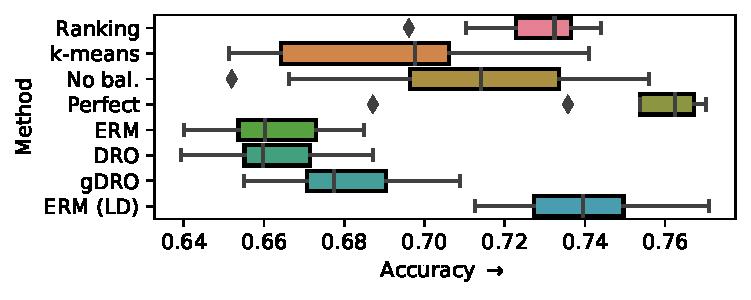
\includegraphics[width=\columnwidth]{figures/adult_partial_acc.pdf}
    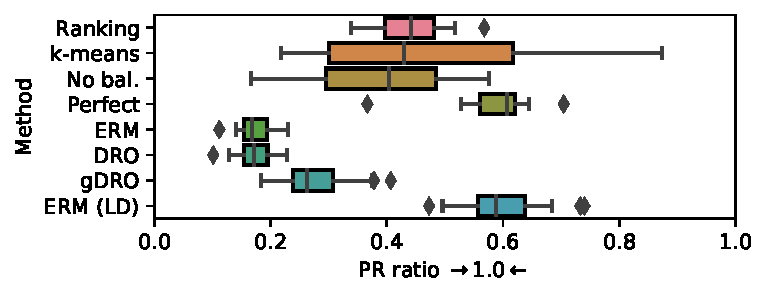
\includegraphics[width=\columnwidth]{figures/adult_partial_prr.pdf}
    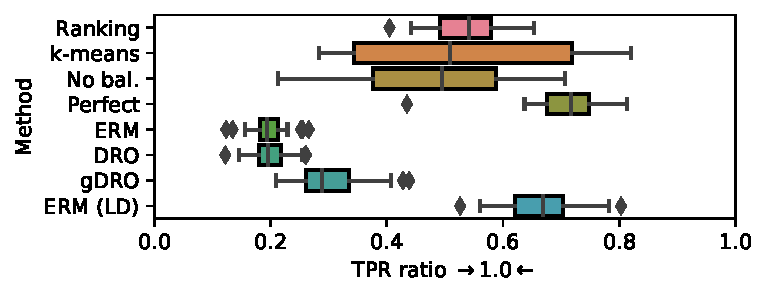
\includegraphics[width=\columnwidth]{figures/adult_partial_tprr.pdf}
    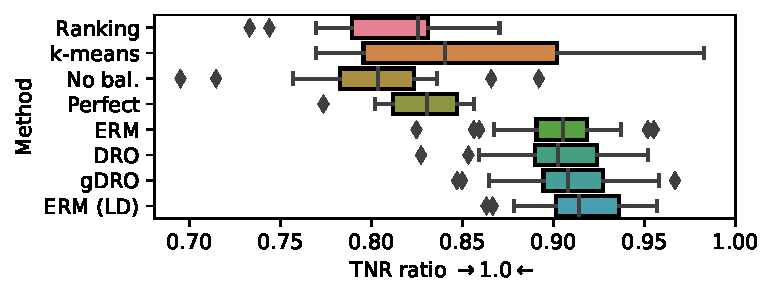
\includegraphics[width=\columnwidth]{figures/adult_partial_tnrr.pdf}
    \caption{%
    Results for the Adult Income dataset with \emph{subgroup bias},
    for the binary classification task of predicting whether an individual earns $>$\$50,000 with a binary subgrouping based on \emph{gender}.
    \texttt{ERM (LD)} refers to a model based on ERM (empirical risk minimization),
    trained on a \emph{l}abelled \emph{d}eployment set; thus not suffering from bias in the training set.
    \textsc{Top left}: Accuracy.
    \textsc{Top right}: Positive rate ratio.
    \textsc{Bottom left}: True positive rate ratio.
    \textsc{Bottom right}: True negative rate ratio.
    For the \texttt{Ranking} clustering, the clustering accuracy was 69.7\% $\pm$ 0.3\%;
    for \texttt{K-means} it was 43\% $\pm$ 3\%.
    }%
    \label{fig:adult-subgroup-bias}
\end{figure*}
\begin{figure*}[p]
    \centering
    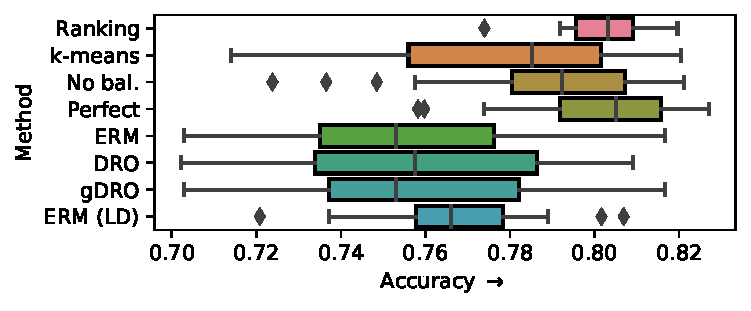
\includegraphics[width=\columnwidth]{figures/adult_miss_s_acc.pdf}
    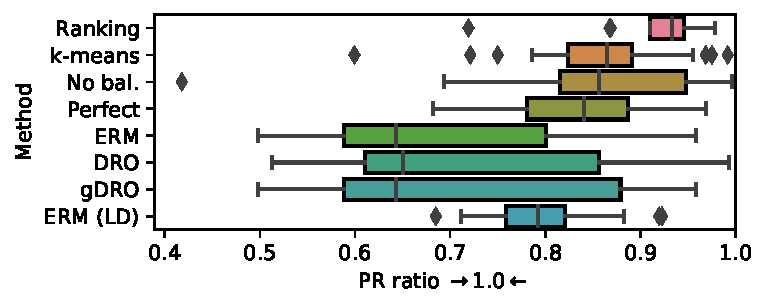
\includegraphics[width=\columnwidth]{figures/adult_miss_s_prr.pdf}
    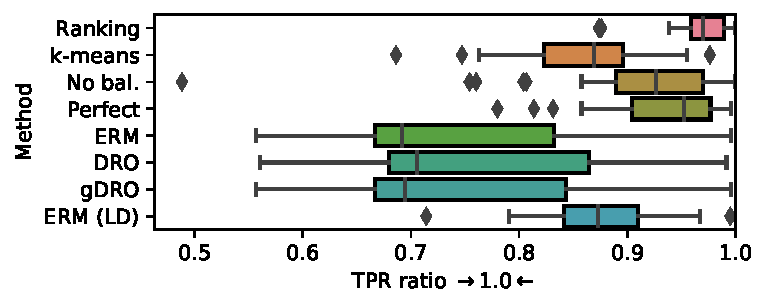
\includegraphics[width=\columnwidth]{figures/adult_miss_s_tprr.pdf}
    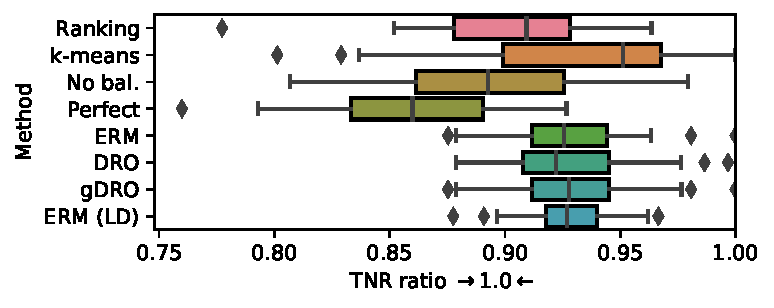
\includegraphics[width=\columnwidth]{figures/adult_miss_s_tnrr.pdf}
    \caption{%
    Results for the Adult Income dataset with a \emph{missing subgroup},
    for the binary classification task of predicting whether an individual earns $>$\$50,000 with a binary subgrouping based on \emph{gender}.
    \texttt{ERM (LD)} refers to a model based on ERM (empirical risk minimization),
    trained on a \emph{l}abelled \emph{d}eployment set; thus not suffering from bias in the training set.
    \textsc{Top left}: Accuracy.
    \textsc{Top right}: Positive rate ratio.
    \textsc{Bottom left}: True positive rate ratio.
    \textsc{Bottom right}: True negative rate ratio.
    For the \texttt{Ranking} clustering, the clustering accuracy was 60.4\% $\pm$ 0.8\%;
    for \texttt{K-means} it was 44\% $\pm$ 3\%.
    }%
    \label{fig:adult-missing-subgroup}
\end{figure*}
Figures~\ref{fig:adult-subgroup-bias} and \ref{fig:adult-missing-subgroup} show results from our method on the Adult Income dataset \cite{Dua:2017}.
This dataset is a common dataset for evaluating fair machine learning models. 
Each instance in the dataset is described by $14$ characteristics including gender, education, marital status, number of work hours per week among others, along with a label denoting income level ($\geq$\$50K or not). 
We transform the representation into $62$ real and binary features along with the subgroup label $s$. %%%%%%%%CHECK THESE VALUES%%%%%%%%%%%% 
The dataset is naturally imbalanced with respect to gender: 30\% of the males are labelled as earning more than \$50K per year (high income), while only 11\% of females are labelled as such.
For further details on the dataset construction, see section~\ref{ssec:dataset-construction-adult}.
%
Following standard practice in algorithmic fairness, e.g. \citet{zemel2013learning}, we consider gender to be the subgroup label $s$.

We study the following two settings.
1) \emph{subgroup bias}: we have labelled training data for males ($s=1$) with both positive and negative outcomes, but for the group of females ($s=0$), we only observe the one-sided negative outcome, so the source $\Omega_{y=1,s=0}$ is missing;
2) \emph{missing subgroup}: we have training data for males with positive and negative outcomes, but do not have labelled data for females, i.e.both \ $\Omega_{y=1,s=0}$ and $\Omega_{y=0,s=0}$ are missing.

As before, \texttt{Ranking}, \texttt{k-means}, \texttt{No bal.}\ and \texttt{Perfect} refer to our method with different procedures for constructing (approximately) perfect bags.
As baseline methods, we have \texttt{ERM} (standard empirical risk minimization with balanced batches), \texttt{DRO} \citep{HasSriNamLia18}, \texttt{gDRO} \citep{sagawa2019distributionally}
and \texttt{ERM (LD)} which is the same model as \texttt{ERM}, but trained on the labelled deployment set, in addition to the training set.

In both settings, we observe the same order as for the other dataset in terms of accuracy: \texttt{Perfect} (with ground truth labels for balancing) achieves the highest performance, followed by \texttt{Ranking}, then \texttt{No bal.}, and finally \texttt{k-means}.
However, for the \emph{missing subgroup} setting, \texttt{Ranking} and \texttt{Perfect} are almost identical and the former performs better in terms of de-biasing metrics.
This decreased reliance on balancing can be explained by the additional supervision that comes with having two sources missing instead of one - in order for the discriminator to distinguish between bags from the deployment set and bags from the training set, the former need only contain \emph{one} of the two missing sources.

Generally, we observe a high variance in the results. This is not attributable to our method, however, with the baselines exhibiting the same behaviour, but rather to the fact that the Adult Income dataset is a very noisy dataset which, at the best of times, allows only about 85\% accuracy to be attained (see also \cite{agrawal2020debiasing}). The problem is that samples vary widely in how informative they are. This, coupled with our artificially biasing the dataset to be even more biased (as \emph{subgroup bias} and \emph{missing subgroup}), makes the achievable performance very dependent on which samples the classifier gets to see, which varies according to the random seed used for the data set split.

\subsection{Dataset Construction}\label{sec:dataset-construction}

\paragraph{Coloured MNIST biasing parameters.}
To simulate a real-word setting where the data, labelled or otherwise, is not naturally balanced, we bias the Coloured MNIST training and deployment sets by downsampling certain colour/digit combinations. The proportions of each such combination \emph{retained} in the \emph{subgroup bias} (in which we have one source missing from the training set) and \emph{missing subgroup} (in which we have two sources missing from the training set) are enumerated in table~\ref{color_mnist_biasing_po} and \ref{color_mnist_biasing_id}, respectively.
For the 3-digit-3-colour variant of the problem, no biasing is applied to either the deployment set or the training set (the missing combinations are specified in the caption accompanying figure~\ref{fig:cmnist-3dig-4miss-add}); this variant was experimented with only under the subgroup-bias setting.

\begin{table}[ht]
\caption{Biasing parameters for the training (left) and deployment (right) sets of Coloured MNIST in the \emph{subgroup bias} setting.}
\label{color_mnist_biasing_po}
\centering
\begin{tabular}{lcc}
\toprule
Combination   & \multicolumn{2}{c}{Proportion retained} \\ \cmidrule(lr){2-3}
  & training set & deployment set \\ \midrule
(y = 2, s = {\color{purple}purple}) & 1.0  & 0.7 \\
(y = 2, s = {\color{green}green})   & 0.3  & 0.4 \\
(y = 4, s = {\color{purple}purple}) & 0.0  & 0.2 \\
(y = 4, s = {\color{green}green})   & 1.0  & 1.0 \\
\bottomrule
\end{tabular}
\end{table}

\begin{table}[ht]
\caption{Biasing parameters for the training (left) and deployment (right) sets of Coloured MNIST in the \emph{missing subgroup} setting.}
\label{color_mnist_biasing_id}
\centering
\begin{tabular}{lcc}
\toprule
Combination   & \multicolumn{2}{c}{Proportion retained} \\ \cmidrule(lr){2-3}
  & training set & deployment set \\ \midrule
(y = 2, s = {\color{purple}purple}) & 0.0  & 0.7 \\
(y = 2, s = {\color{green}green})   & 0.85 & 0.6 \\
(y = 4, s = {\color{purple}purple}) & 0.0  & 0.4 \\
(y = 4, s = {\color{green}green})   & 1.0  & 1.0 \\
\bottomrule
\end{tabular}
\end{table}

\paragraph{Adult Income.}\label{ssec:dataset-construction-adult}
For the Adult Income dataset, we do not need to apply any synthetic biasing as the dataset naturally contains some bias wrt $s$. Thus, we instantiate the deployment set as just a random subset of the original dataset. Explicit balancing of the test set is needed to yield meaningful evaluation, however, namely in the penalizing of biased classifiers, but need be taken in doing so. Balancing the test set such that
\begin{align}
    |\{x \in X |s=0, y=0\}| &= |\{x \in X |s=1, y=0\}|    \nonumber\\
    \text{and}~|\{x \in X |s=0, y=1\}| &= |\{x \in X |s=1, y=1\}|
\end{align}
where for both target classes, $y=0$ and $y=1$, the proportions of the groups $s=0$ and $s=1$ are made to be the same, is intuitive, yet at the same time precludes sensible comparison of the accuracy/fairness trade-off of the different classifiers.
Indeed, with the above conditions, a majority classifier (predicting all 1s or 0s) achieves comparable accuracy to the fairness-unaware baselines, while also yielding perfect fairness, by construction.
This observation motivated us to devise an alternative scheme, where we balance the test set according to the following constraints
\begin{align}
    & |\{x \in X |s=0, y=0\}| 
    = |\{x \in X |s=0, y=1\}|  \nonumber \\
    = &|\{x \in X |s=1, y=1\}|
    = |\{x \in X |s=1, y=0\}|~.
 \end{align}
That is, all subsets of $\gS \times \gY$ are made to be equally sized. Under this new scheme the accuracy of the the majority classifier is 50\% for the binary-classification task.


\subsection{Optimization}
\begin{table*}[p]
 \centering
 \caption{Selected hyperparameters for experiments with Coloured MNIST, Adult and CelebA datasets.}
 \label{tab:hparams}
\scalebox{0.65}{
 \begin{tabular}{llll}
 \toprule
 & \textsc{Coloured MNIST} & \textsc{Adult} & \textsc{CelebA}       
 \\ & 2-dig SB / 2-dig MS / 3-dig SB
 \\ \midrule
 Input size  &   $3 \times 32 \times 32$ & $61$ & $3 \times 64 \times 64$ \\  \midrule
 \multicolumn{4}{c}{Autoencoder}                     \\ \midrule
 Levels                      & $4$         & $1$    & $5$\\
 Level depth                 & $2$         & $1$    & $2$\\
 Hidden units / level        & $[32, 64, 128, 256]$ & $[61]$ & $[32, 64, 128, 256, 512]$\\
 Activation                  & GELU        & GELU   & GELU   \\
 Downsampling op.  & Strided Convs. & -- & Strided Convs.\\
 Reconstruction loss         & MSE         & Mixed$^1$  & MSE \\
 Learning rate               & $1 \times 10^{-3}$   & $1 \times 10^{-3}$  & $1 \times 10^{-3}$ \\ \midrule
 \multicolumn{4}{c}{Clustering}                      \\ \midrule
 Batch size                  & $256$      & $1000$  & --\\
 AE pre-training epochs      & $150$        & $100$ & --   \\
 Clustering epochs           & $100$       & $300$  & -- \\
 Self-supervised loss & Cosine + BCE & Cosine + BCE & --\\
 U (for ranking statistics)             & $5$         & $3$     & --    \\   \midrule
 \multicolumn{4}{c}{Distribution Matching}                   \\ \midrule
 Batch size & $1$/$32$/$14$  & $64$   & $32$ \\
 Bag size   & $256$/$8$/$18$ & $32$ & $8$ \\
 Training iterations    & $8\text{k}/8\text{k}/20\text{k}$ & $5\text{k}$ & $15\text{k}$ \\
 Encoding ($z$) size$^2$  & $128$   & $35$  & $128$ \\
 Binarised $z_s$ & {\boxedsymbols ✗}\, / \cmark\, / \cmark & \xmark & \xmark \\
 $y$-predictor weight ($\lambda_1$) & $1$ & $0$ & $1$  \\ 
 $s$-predictor weight ($\lambda_2$) & $1$ & $0$ & $0$  \\ 
 Adversarial weight ($\lambda_3$)   & $1 \times
 10^{-3}$   & $1$   & $1$\\ 
 Stopgradient $\left(\nabla_\theta h_\psi(f_\theta(X^\mathit{dep}))=0\right)$ & \xmark & \cmark & \xmark \\
 \midrule
 \multicolumn{4}{c}{Predictors}   \\ \midrule
 Learning rate  & $3 \times 10^{-4}$ &   $1 \times 10^{-3}$  $ 1 \times 10^{-3}$\\
 \midrule
 \multicolumn{4}{c}{Discriminator}                   \\ \midrule
 Attention mechanism$^3$    & Gated   & Gated & Gated \\
 Hidden units pre-aggregation  & $[256, 256]$  & $[32]$ & $[256, 256]$\\
 Hidden units post-aggregation & $[256, 256]$ & --  & $[256, 256]$ \\
 Embedding dim (for attention) & $32$ & $128$ & $128$ \\
 Activation & GELU & GELU & GELU \\
 Learning rate  & $3 \times 10^{-4}$    & $1 \times 10^{-3}$ & $1 \times 10^{-3}$\\
 Updates / AE update    & $1$  & $3$    & $1$    \\
 \bottomrule
 \multicolumn{4}{l}{\footnotesize $^1$ Cross-entropy is used for categorical features, MSE for continuous features.} \\
  \multicolumn{4}{p{\textwidth}}{\footnotesize $^2$ $|z|$ denotes the combined size of $z_s$ and $z_y$, with the former occupying $\ceil{\text{log}_2(\mathcal{S})}$ dimensions, the latter the remaining } \\
  \multicolumn{4}{p{\textwidth}}{\footnotesize dimensions.} \\
  \multicolumn{4}{p{\textwidth}}{\footnotesize $^3$ The attention mechanism used for computing the sample-weights within a bag. \emph{Gated} refers to gated attention  proposed by
%   \cite{ilse2018attention}, while \emph{SDP} refers to the scaled dot-product attention proposed by \cite{vaswani2017attention}.
  } \\ 
  \multicolumn{4}{p{\textwidth}}{\footnotesize  \cite{ilse2018attention}.} \\ 
 \end{tabular}
}
\end{table*}

The hyperparameters and architectures for the Autoencoder (\texttt{AE}), Predictor and Discriminator subnetworks used for the experiments with all datasets are detailed in Table \ref{tab:hparams}. All networks are trained using the Adam optimiser \citep{kingma2015adam}.

For the Coloured MNIST and CelebA datasets, the baseline \texttt{CNN}, \texttt{DRO}, and \texttt{LfF} (in the case of the former) models use an architecture identical to that of the encoder with two exceptions: 1) max-pooling being used for spatial downsampling instead of strided convolutions; 2) the final convolutional layer is followed by a global average pooling layer followed by a fully-connected classification layer. For evaluating our method, we simply train a linear classifier on top of $z_y$; this is sufficient due to linear-separability being enforced during training by the $y$-predictor.
For the Adult Income dataset, we use an MLP made up of a single hidden layer 35 units in size, followed by a SELU activation \citep{klambauer2017self}, as both both the downstream classifier for our method, and as the network architecture of the baselines. 
All baselines and downstream classifiers alike were trained for $60$ epochs with a learning rate of $1 \times 10^{-3}$ and a batch size of $256$.

Since, by design, we do not have labels for all subgroups the model will be tested on, and bias against these missing subgroups is what we aim to avoid, properly validating, and thus conducting hyperparameter selection for models generally, is not straightforward.
We can use estimates of the mutual information between the learned-representation and $s$ and $y$ (which we wish to minimise w.r.t.\ to the former, maximise w.r.t.\ the latter) to guide the process, though optimizing the model w.r.t.\ to these metrics obtained from only the training set does not guarantee generalization to the missing subgroups.
We can, however, additionally measure the entropy of the predictions on the encoded test set and seek to maximise it across all samples, or alternatively train a discriminator of the same kind used for distribution matching as a measure the shift in the latent space between datasets.
We use the latter approach (considering, the learned distance between subspace distributions, accuracy, and reconstruction loss) to inform an extensive grid-search over the hyperparameter space of our model.

For the \texttt{DRO} baseline, we allowed access to the labels of the test set for the purpose of hyperparameters selection, performing a grid-search over multiple splits to avoid overfitting to any particular instantiation.
Specifically, the threshold ($\eta$) parameter for \texttt{DRO} was determined by a grid-search over the space $\{0.01, 0.1, 0.3, 1.0\}$. The same procedure was carried out for selecting the model capacity constant ($C$) of the related \texttt{gDRO} baseline.

In addition to the losses stated in the distribution matching objective, $\mathcal{L}$, in the main text, we also regularise the encoder by the $\ell^2$ norm of its embedding, multiplied by a small pre-factor, finding this to work better than more complex regularization methods, such as spectral normalization \citep{miyato2018spectral}, for stabilizing training.

\subsection{Visualizations of results}\label{sec:qual-results}
Figures~\ref{fig:attn_maps} and \ref{fig:cmnist-recon} show some additional visualizations for our results.
For details, see the captions.
\begin{figure*}[tb]
  \centering
    % \begin{subfigure}[b]{0.49\textwidth}
    
\includegraphics[width=0.9\textwidth]{figures/celeba_attn_map.png}
    % \end{subfigure}
    % \hfill
    % \begin{subfigure}[b]{0.49\textwidth}
    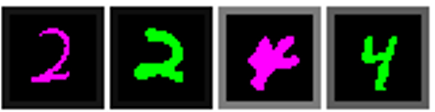
\includegraphics[width=0.9\textwidth]{figures/cmnist_attn_map.png}
    % \end{subfigure}
  \caption{
    Example sample-wise attention maps for bags of CelebA (left) and Coloured MNIST (right) images sampled from a balanced deployment set. The training set is biased according to the SB setting where for CelebA ``smiling females'' constitute the missing source and for Colored MNIST {\color{purple}purple} fours constitute the missing source. The attention weights are used during the discriminator's aggregation step to compute a weighted sum over the bag. The attention-weight assigned to each sample is proportional to the lightness of its frame, with black signifying a weight of 0, white a weight of 1. Those samples belonging to the missing subgroup are assigned the highest weight as they signal from which dataset (training vs. deployment) the bag containing them was drawn from.
  }%
  \label{fig:attn_maps}
\end{figure*}

% \subsection{Qualitative results}\label{sec:qual-results}
\begin{figure*}[tb]
  \centering
  \begin{subfigure}[b]{0.39\textwidth}
    \centering
    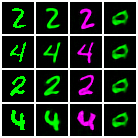
\includegraphics[width=\textwidth]{example_images/fresh-dawn-2179_train_reconstructions_9900.png}
    \caption{
    Different reconstructions on the training set.
    Corresponding to: original, full reconstruction, reconstruction of $z_y$, reconstruction of $z_s$.
    }%
    \label{fig:cmnist-recon-training}
  \end{subfigure}
  % \hfill
  \quad
  \begin{subfigure}[b]{0.39\textwidth}
    \centering
    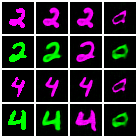
\includegraphics[width=\textwidth]{example_images/fresh-dawn-2179_context_reconstructions_9900.png}
    \caption{
    Different reconstructions on the deployment set.
    Corresponding to: original, full reconstruction, reconstruction of $z_y$, reconstruction of $z_s$.
    }%
    \label{fig:cmnist-recon-deployment}
  \end{subfigure}
  \caption{
   Visualization of our method's solutions for the Coloured MNIST dataset, with {\color{purple}purple} as the missing subgroup.
   In each of the subfigures \ref{fig:cmnist-recon-training} and \ref{fig:cmnist-recon-deployment}:
   Column 1 shows the original images from $x$ from the respective set.
   Column 2 shows plain reconstructions generated from $x_\textit{recon}=g(f_y(x), f_s(x))$.
   Column 3 shows reconstruction with zeroed-out $z_s$: $g(f_y(x), 0)$, which effectively visualises $z_y$.
   Column 4 shows the result of an analogous process where $z_y$ was zeroed out instead.
  }%
  \label{fig:cmnist-recon}
\end{figure*}
% Given a learned invariant representation, we can generate a reconstruction to visualise the information contained in it.
% An example of this can be seen in \figref{fig:3dig-examples}.
% This is from our experiment with 3 digits in Colored MNIST.
% We can clearly see that the reconstructed invariant representation has lost all color information;
% instead all digits are magenta-colored, which was the majority color in the training set.

\subsection{Code}
The code will be published at the following URL: \url{https://github.com/predictive-analytics-lab/fair-dist-matching}.
Instructions on how to run them can be found in the \texttt{README.md}.

\subsection{Additional metrics}
Figures~\ref{fig:cmnist-2v4-partial-add}, \ref{fig:cmnist-2v4-miss-s-add},  and \ref{fig:celeba-gender-smiling-add} show the true positive rate (TPR) ratio and the true negative rate (TNR) ratio as additional metrics for Coloured MNIST (2 digits) and CelebA.
These are computed as the ratio of TPR (or TNR) on subgroup $s=0$ over the TPR (or TNR) on subgroup $s=1$; if this gives a number greater than 1, the inverse is taken.
Similarly to the PR ratio reported in the main paper, these ratios give an indication of how much the prediction of the classifier depends on the subgroup label $s$.

Figure~\ref{fig:cmnist-3dig-4miss-add} shows metrics specific to multi-valued $s$ (\ie, non-binary $s$).
We report the minimum (i.e. farthest away from 1) of the pairwise ratios (PR/TPR/TNR ratio min) as well as the largest difference between the raw values (PR/TPR/TNR diff max) . 
Additionally, we compute the Hirschfeld-Gebelein-R\'enyi (HGR) maximal correlation \citep{renyi1959measures} between $S$ and $Y$, serving as a measure of dependence defined between two variables with arbitrary support.
\begin{figure*}[htp]
  \centering
%   \includegraphics[width=\columnwidth]{figures/cmnist_2v4_partial_acc.pdf}
%   \includegraphics[width=\columnwidth]{figures/cmnist_2v4_partial_pr.pdf}
%   \includegraphics[width=\columnwidth]{figures/cmnist_2v4_partial_tpr.pdf}
%   \includegraphics[width=\columnwidth]{figures/cmnist_2v4_partial_tnr.pdf}
  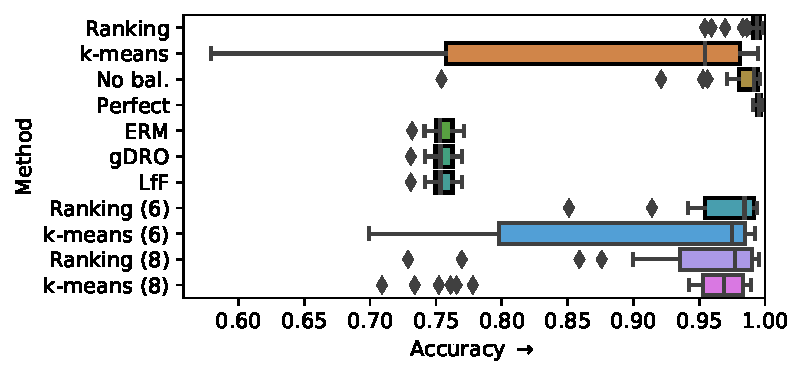
\includegraphics[width=0.8\columnwidth]{figures/cmnist_2v4_partial_overcluster_acc.pdf}
  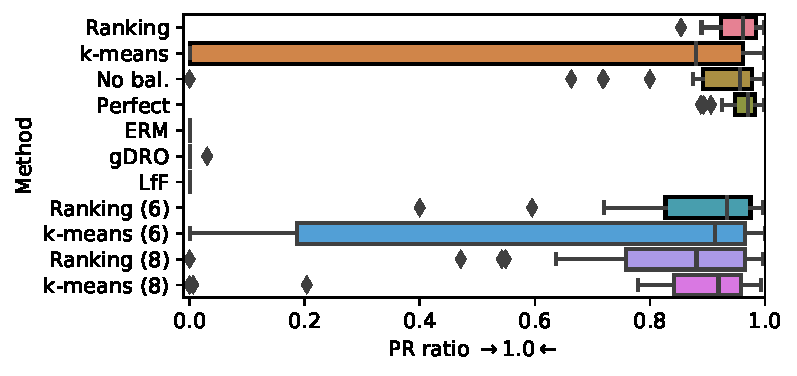
\includegraphics[width=0.8\columnwidth]{figures/cmnist_2v4_partial_overcluster_prr.pdf}
  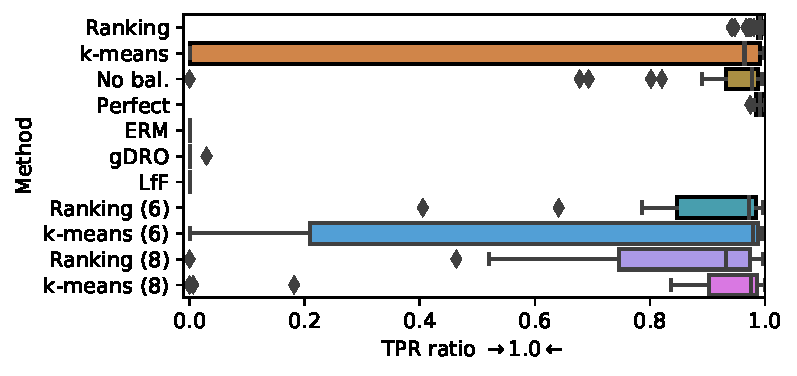
\includegraphics[width=0.8\columnwidth]{figures/cmnist_2v4_partial_overcluster_tprr.pdf}
  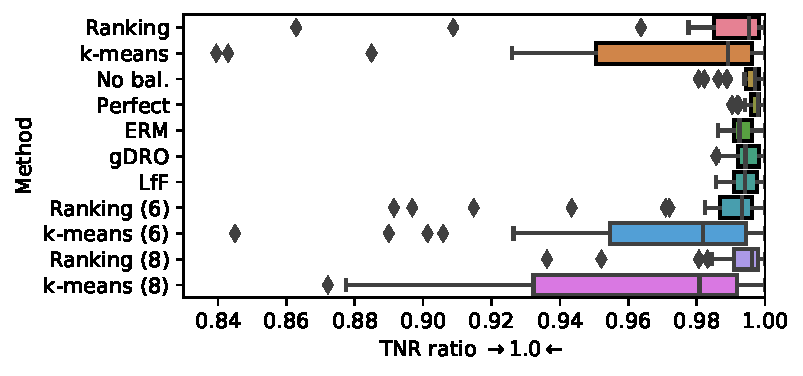
\includegraphics[width=0.8\columnwidth]{figures/cmnist_2v4_partial_overcluster_tnrr.pdf}
  \caption{
    Results from 30 repeats for the Coloured MNIST dataset with two digits, 2 and 4, with \emph{subgroup bias} for the colour `{\color{purple}purple}': for {\color{purple}purple}, only the digit class `2' is present.
    \textsc{Top left}: Accuracy.
    \textsc{Top right}: Positive rate ratio.
    \textsc{Bottom left}: True positive rate ratio.
    \textsc{Bottom right}: True negative rate ratio.
    For the \texttt{Ranking} clustering, the clustering accuracy was 96\% $\pm$ 6\%;
    for \texttt{K-means} it was 64\% $\pm$ 10\%.
    For an explanation of \texttt{Ranking (8)} and \texttt{K-means (8)} see section~\ref{sec:overclustering}.
  }%
  \label{fig:cmnist-2v4-partial-add}
\end{figure*}
\begin{figure*}[htp]
  \centering
%   \includegraphics[width=\columnwidth]{figures/cmnist_2v4_miss_s_alt_acc.pdf}
%   \includegraphics[width=\columnwidth]{figures/cmnist_2v4_miss_s_alt_pr.pdf}
%   \includegraphics[width=\columnwidth]{figures/cmnist_2v4_miss_s_alt_tpr.pdf}
%   \includegraphics[width=\columnwidth]{figures/cmnist_2v4_miss_s_alt_tnr.pdf}
  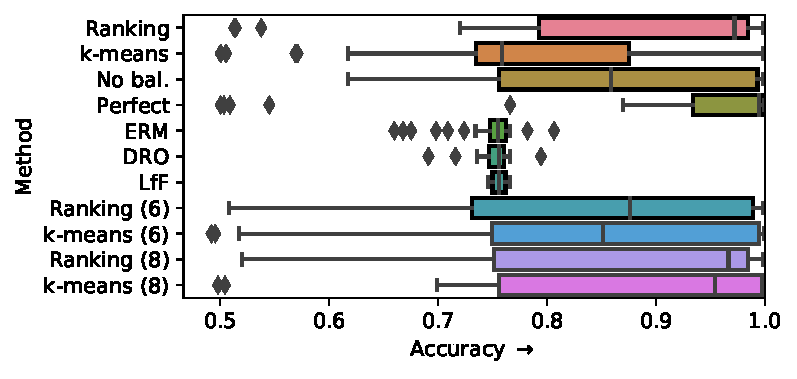
\includegraphics[width=0.8\columnwidth]{figures/cmnist_2v4_miss_s_overcluster_acc.pdf}
  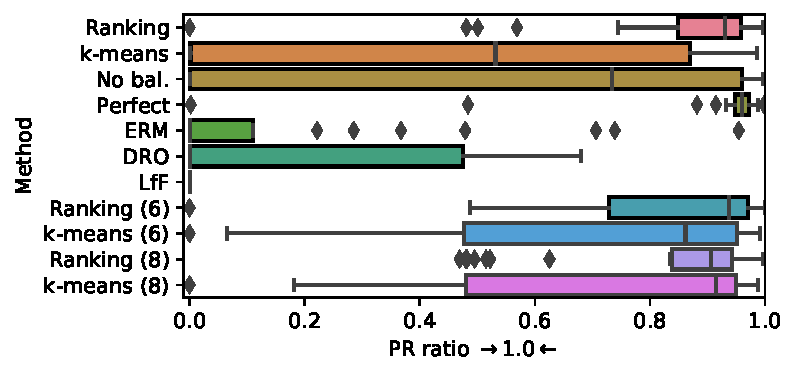
\includegraphics[width=0.8\columnwidth]{figures/cmnist_2v4_miss_s_overcluster_prr.pdf}
  \includegraphics[width=0.8\columnwidth]{figures/cmnist_2v4_miss_s_overcluster_tprr.pdf}
  \includegraphics[width=0.8\columnwidth]{figures/cmnist_2v4_miss_s_overcluster_tnrr.pdf}
  \caption{
    Results from 30 repeats for the Coloured MNIST dataset with two digits, 2 and 4, with a \emph{missing subgroup}: the training dataset only has {\color{green}green} digits.
    \textsc{Top left}: Accuracy.
    \textsc{Top right}: Positive rate ratio.
    \textsc{Bottom left}: True positive rate ratio.
    \textsc{Bottom right}: True negative rate ratio.
    For the \texttt{Ranking} clustering, the clustering accuracy was 88\% $\pm$ 5\%;
    for \texttt{K-means} it was 72\% $\pm$ 16\%.
    For an explanation of \texttt{Ranking (8)} and \texttt{K-means (8)} see section~\ref{sec:overclustering}.
  }%
  \label{fig:cmnist-2v4-miss-s-add}
\end{figure*}
\begin{figure*}[htp]
  \centering
%   \includegraphics[width=\columnwidth]{figures/cmnist_3dig_4miss_hgr.pdf}\\
  \includegraphics[width=0.8\columnwidth]{figures/cmnist_3dig_4miss_prr-min.pdf}
  \includegraphics[width=0.8\columnwidth]{figures/cmnist_3dig_4miss_prd-max.pdf}
  \includegraphics[width=0.8\columnwidth]{figures/cmnist_3dig_4miss_tprr-min.pdf}
  \includegraphics[width=0.8\columnwidth]{figures/cmnist_3dig_4miss_tprd-max.pdf}
  \includegraphics[width=0.8\columnwidth]{figures/cmnist_3dig_4miss_tnrr-min.pdf}
  \includegraphics[width=0.8\columnwidth]{figures/cmnist_3dig_4miss_tnrd-max.pdf}
  \caption{
    Results from 30 repeats for the Coloured MNIST dataset with three digits: `2', `4' and `6'.
    Four combinations of digit and colour are missing: {\color{green}green} 2's, {\color{blue}blue} 2's, {\color{blue}blue} 4's and {\color{green}green} 6's.
    % \textsc{First row}: Hirschfeld-Gebelein-R\'enyi maximal correlation between $S$ and $Y$.
    \textsc{First row, left}: minimum of all positive rate ratios.
    \textsc{First row, right}: maximum of all positive rate differences.
    \textsc{Second row, left}: minimum of all true positive rate ratios.
    \textsc{Second row, right}: maximum of all true positive rate differences.
    \textsc{Third row, left}: minimum of all true negative rate ratios.
    \textsc{Third row, right}: maximum of all true negative rate differences.
  }%
  \label{fig:cmnist-3dig-4miss-add}
\end{figure*}
\begin{figure*}[htp]
  \centering
%   \includegraphics[width=\columnwidth]{figures/celeba_gender_smiling_acc.pdf}
%   \includegraphics[width=\columnwidth]{figures/celeba_gender_smiling_pr.pdf}
  \includegraphics[width=\columnwidth]{figures/celeba_gender_smiling_tprr.pdf}
  \includegraphics[width=\columnwidth]{figures/celeba_gender_smiling_tnrr.pdf}
  \caption{
    Results from 10 repeats for the CelebA dataset with the \emph{subgroup bias} setting.
    The task is to predict ``smiling'' vs ``non-smiling'' and the subgroups are based on gender.
    The subgroup ``female'' is missing samples for the ``smiling'' class.
    % \textsc{Top left}: Accuracy.
    % \textsc{Top right}: Positive rate ratio.
    \textsc{Left}: True positive rate ratio.
    \textsc{Right}: True negative rate ratio.
  }%
  \label{fig:celeba-gender-smiling-add}
\end{figure*}

\subsection{Clustering with an incorrect number of clusters}\label{sec:overclustering}
We also investigate what happens when the number of clusters is set incorrectly.
For 2-digit Coloured MNIST, we expect 4 clusters, corresponding to the 4 possible combinations of the binary class label $y$ and the binary subgroup label $s$.
However, there might be circumstances where the correct number of clusters is not known; how does the batch balancing work in this case?
We run experiments with the number of clusters set to 6 and to 8, while otherwise not changing any part of the method.
It should be noted that this is a very na\"ive way of dealing with an unknown number of clusters.
There are methods specifically designed for identifying the right number of clusters \citep{hamerly2004learning,chazal2013persistence},
and that is what would be used if this situation came up in practice.

The results can be found in figures~\ref{fig:cmnist-2v4-partial-add} and \ref{fig:cmnist-2v4-miss-s-add}.
Bags and batches are constructed by drawing an equal number of samples from each cluster.
Unsurprisingly, the method performs worse than with the correct number of clusters.
When investigating how the clustering methods deal with the larger number of clusters,
we found that it is predominantly those samples that do not appear in the training set
which get spread out among the additional clusters.
This is most likely due to the fact that the clustering is semi-supervised,
with those clusters that occur in the training set having supervision.
The overall effect is that the samples which are not appearing in the training set are overrepresented in the drawn bags,
which means it is easier for the adversary to identify where the bags came from,
and the encoder cannot properly learn to produce an invariant encoding.

% \begin{table*}[tp]
%   \centering
%   \caption{
%     Results on Colored MNIST dataset for a 3-digits-3-colors task, i.e. classification of the digits \emph{two} versus \emph{four} vs \emph{six} with a protected attribute that can take three values ({\color{purple}purple}, {\color{green}green}, {\color{blue}blue}).
%     We consider the scenarios of learning with subgroup bias with four sources missing (30 repeats). 
%   }
%   \label{tab:colormnist3_sup}
%   \scalebox{0.79}{
%   \begin{tabular}{lccccccc}
%     \hline
%     \multicolumn{6}{c}{}\\
%     \multicolumn{6}{c}{Learning with subgroup bias, the sources
%     $\mathcal{M}_{y=\text{'two'},s=\color{green}green}$,
%     $\mathcal{M}_{y=\text{'two'},s=\color{blue}blue}$,
%     $\mathcal{M}_{y=\text{'four'},s=\color{blue}blue}$ and
%     $\mathcal{M}_{y=\text{'six'},s=\color{green}green}$
%     are invisible.}\\
%     \multicolumn{6}{c}{}\\
%     \hline
%     %
%                                          &         AR min. ratio& TPR min. ratio & TNR min. ratio &   AR max. diff &  TPR max. diff &   TNR max. diff \\
%                              \texttt{ZSF} &    0.604 $\pm$ 0.213 &  0.866 $\pm$ 0.176 &  0.702 $\pm$ 0.292 &  0.236 $\pm$ 0.189 &  0.133 $\pm$ 0.175 &  0.297 $\pm$ 0.291 \\
%  \texttt{DRO \cite{HasSriNamLia18}} &     0.027 $\pm$ 0.05 &  0.077 $\pm$ 0.145 &  0.128 $\pm$ 0.147 &  0.887 $\pm$ 0.101 &  0.923 $\pm$ 0.145 &  0.871 $\pm$ 0.147 \\
%   \texttt{Kamiran \& Calders (2012) CNN} &    0.072 $\pm$ 0.077 &  0.208 $\pm$ 0.217 &  0.039 $\pm$ 0.054 &  0.904 $\pm$ 0.087 &  0.792 $\pm$ 0.217 &  0.961 $\pm$ 0.054 \\
%     \hline
%     \hline
%   \end{tabular}}
% \vspace{-0.5cm}
% \end{table*}
% \bibliography{bibfile}
% \bibliographystyle{icml2021}
% \end{document}


% In the unusual situation where you want a paper to appear in the
% references without citing it in the main text, use \nocite

% \bibliography{bibfile}
% \bibliographystyle{icml2021}


% \end{document}


% This document was modified from the file originally made available by
% Pat Langley and Andrea Danyluk for ICML-2K. This version was created
% by Iain Murray in 2018, and modified by' Alexandre Bouchard in
% 2019 and 2021. Previous contributors include Dan Roy, Lise Getoor and Tobias
% Scheffer, which was slightly modified from the 2010 version by
% Thorsten Joachims & Johannes Fuernkranz, slightly modified from the
% 2009 version by Kiri Wagstaff and Sam Roweis's 2008 version, which is
% slightly modified from Prasad Tadepalli's 2007 version which is a
% lightly changed version of the previous year's version by Andrew
% Moore, which was in turn edited from those of Kristian Kersting and
% Codrina Lauth. Alex Smola contributed to the algorithmic style files.
